%%%%%%%% ICML 2026 SUBMISSION FILE %%%%%%%%%%%%%%%%%
\documentclass{article}

% Recommended packages
\usepackage{microtype}
\usepackage{graphicx}
\usepackage{booktabs}
\usepackage{pifont}
\usepackage{xspace}
\usepackage{enumitem}

% ICML style (avoid hyperref clashes for submission)
\usepackage{icml2025}
\usepackage{hyperref}
% Math + refs
\usepackage{amsmath,amssymb,mathtools,amsthm}
\usepackage[capitalize,noabbrev]{cleveref}

% Figures
\usepackage{subcaption} % (replaces deprecated subfigure)
\usepackage{tikz}
\usetikzlibrary{arrows.meta,positioning,fit,calc}

\graphicspath{{plots/}{.}} % includes current dir for provided images

\usepackage{tikz}
\usepackage{amsmath}
\usetikzlibrary{arrows.meta,decorations.pathreplacing,calc}

\newcommand{\ye}[1]{\textcolor{purple}{(Yanai:) #1}}

% Theorems (statements in main; proofs in appendix)
\theoremstyle{plain}
\newtheorem{theorem}{Theorem}[section]
\newtheorem{lemma}[theorem]{Lemma}
\newtheorem{proposition}[theorem]{Proposition}
\theoremstyle{definition}
\newtheorem{definition}[theorem]{Definition}
\theoremstyle{remark}
\newtheorem{remark}[theorem]{Remark}
\usepackage{gensymb}

% -------------------------
% Minimal, consistent notation
% -------------------------
% \newcommand{\LN}{\mathrm{LN}}
% \newcommand{\E}{\mathbb{E}}
% \newcommand{\Var}{\mathrm{Var}}
% \newcommand{\R}{\mathbb{R}}
% \newcommand{\V}{\mathcal{V}}

% Optional: visually emphasize key terms
% \newcommand{\term}[1]{\textbf{#1}}

\icmltitlerunning{Position Without Positional Embeddings}

\begin{document}

\twocolumn[
\icmltitle{Position Without Positional Embeddings:\\
A Geometric Gauge in NoPE Transformers}

\begin{icmlauthorlist}
\icmlauthor{Matan Avitan}{biu}
\icmlauthor{Ido Nachum}{haifa}
\icmlauthor{Yoav Goldberg}{biu,ai2}
\end{icmlauthorlist}

\icmlaffiliation{biu}{Bar-Ilan University, Ramat Gan, Israel}
\icmlaffiliation{haifa}{University of Haifa, Haifa, Israel}
\icmlaffiliation{ai2}{Allen Institute for Artificial Intelligence}

\icmlcorrespondingauthor{Matan Avitan}{matan13av@gmail.com}

\icmlkeywords{transformers, positional encoding, mechanistic interpretability, causal attention}

\vskip 0.3in
]

% \printAffiliationsAndNotice{}

%%%%%%%%%%%%%%%%%%%%%%%%%%%%%%%%%%%%%%%%%%%%%%%%%%%%%%%%%%%%%%%%%%%%%%%%%%%%%%%
\begin{abstract}

Transformers are typically coupled with positional embeddings that explicitly encodes tokens' position. However, prior work has shown empirical evidence that transformers with no-position embedding (NoPE) work well in practice, while having no such explicit information, which is crucial for the language modeling task.
While previous work showed how the causal attention creates position-dependent variance, it ignored the LayerNorm which is commonly used in transformer models, which allegedly erases the position information.
In this work, we find a circuit that encodes the position information in NoPE transformers. We demonstrate the ability of such circuit to encode positional information in a simple model with only two transformer blocks. Interestingly, we demonstrate how the position information survives the layer norm through the direction, rather than the magnitude.
Then, we demonstrate how the mechanism we discovered is implemented in a transformer model that predicts the position, in two separate training setups.


% How do causal Transformers without positional embeddings (NoPE) recover \emph{absolute position}?
% Prior work showed that causal attention creates position-dependent variance, but this explanation is incomplete:
% LayerNorm erases variance information by normalizing each sample.

% We identify a complete \term{geometric gauge} mechanism in a minimal two-block NoPE Transformer trained on position regression.
% The circuit has five steps: (1) the causal mask structurally prevents position 0 from averaging, preserving its representation norm;
% (2) learned value/output projections amplify position 0 by $3\times$ and create \emph{opposite} directions for position-0 and non-position-0 contributions;
% (3) learned query-key weights create strong attention to position 0;
% (4) as position increases, the attention output smoothly rotates from the position-0 direction toward the ``others'' direction;
% (5) a linear head aligned with the others direction reads this rotation.

% We validate this circuit through write-subspace interventions, showing that position decoding flows through a low-rank bottleneck
% ($r_{95}=2$ for a single-head model).
% The mechanism explains both why position information survives LayerNorm (it is carried by \emph{direction}, not magnitude)
% and why the model extrapolates to longer sequences (the rotation is length-agnostic when anchored to position 0).
\end{abstract}

%%%%%%%%%%%%%%%%%%%%%%%%%%%%%%%%%%%%%%%%%%%%%%%%%%%%%%%%%%%%%%%%%%%%%%%%%%%%%%%
\section{Introduction}
%%%%%%%%%%%%%%%%%%%%%%%%%%%%%%%%%%%%%%%%%%%%%%%%%%%%%%%%%%%%%%%%%%%%%%%%%%%%%%%

Transformers typically inject explicit positional information~\citep{vaswani2017attention, wang2021rotary, alibi}, as this is a crucial information for the language modeling task, and it is not clear how token position can be extracted otherwise.
Yet, prior work have \textit{empirically} shown that causal Transformers can represent absolute position even when positional embeddings are removed, termed NoPE - No Position Embeddings~\citep{haviv2022transformer, chi-etal-2023-latent, kazemnejad2023lenghGeneralization}.
A common explanation is that causal attention mixes an increasingly long prefix, so the variance of the attention aggregate decreases with position \citep{chi-etal-2023-latent}.
However, this explanation is incomplete.
LayerNorm \citep{ba2016layer} normalizes each sample to zero mean and unit variance, so per-sample variance cannot directly carry position information. Thus, an open question that remains is \textit{how transformer models can encode position information in NoPE?}
% What survives LayerNorm is \emph{direction}---and this is exactly where we find the mechanism.

% \paragraph{Our contribution.}
In this work, we identify a circuit \citep{elhage2021mathematical} in a 2-block transformer that encodes position. The circuit, which we term
a \term{geometric gauge}, explains how NoPE Transformers encode position through a directional rotation between the BOS-direction and the mean non-BOS direction as position increases.
At the core of the mechanism, the position information is encoded by considering two directions: the direction of the BOS token which is fixed across the sequence, and the direction of the average embedding vectors of the other tokens in the prefix, which changes. The residual stream vector is a mix of these two directions. Later layers can then read the difference between these two direction, which grows as the sequence length increases.
We can think of the two directions as two ends of a gauge, one fixed and one moving by a fixed amount at each time step, where the position is read by measuring the angle between them. We thus call this mechanism a \emph{geometric gauge}.
Concretely, with randomly initialized embeddings, the causal attention mechanism induces a \textit{position bias}, where the residual stream's norm of the first token after the first transformer block is large, compared to all other tokens' norms. Then, the attention in the second transformer block assigns more attention and a larger norm to the first token (BOS). Moreover the multiplication by $W_OW_V$ orient the BOS token in a direction that is well-seperated --- often nearly opposite --- from the direction of non-BOS tokens. Therefore, this bias creates a 2-dimensional subspace that separates the first token compared to all other tokens, whose representations converge to the same vector in this 2-dimensional subspace. Finally, by multiplying the residual stream after the second transformer block with the regression head, whose vector is aligned with the no-BOS tokens direction, the model can accurately predict the position of a token.

After establishing the ability of a NoPE transformer to encode position information through the \textit{geometric gauge} mechanism, we provide evidence that this is the learned mechanism in two experiments. The first experiment relies on a simple transformer with a single attention head, where all weights are frozen except for the second attention and the regression head. In the second experiment, we use the same 2-block transformer model, but with 12 heads, and all of the weights are trained. These experiments, together with a causal analysis of the models show that the learned mechanism correspond to our hypothesized circuit, and provides concrete evidence that NoPE transformers can learn to extract positional information.


\ye{something about the theoretical part}

Overall, this paper is organized as follows. We start by discussing prior work (\S\ref{sec:background}), and establishing the notation used in this work (\S\ref{sec:notation}). Then, we propose the \textit{Geometric Gauge} circuit, and how a two-block transformer can encode position information (\S\ref{sec:mechanism_text}). Then, we empirically show how two trained NoPE transformers learn the geometric gauge mechanism (\S\ref{sec:empirical}).
Finally, we discuss how the \textit{geometric gauge} circuit related to @@@ (\S\ref{sec:theory}), and end with a discussion of our findings (\S\ref{sec:}).\footnote{We will release the code developed for this work upon publication.}

% This achieves $R^2 = 0.993$ position prediction with \emph{one} attention head.
% We validate the mechanism through write-subspace interventions, showing that only 2 singular directions of the write map $B = W_O W_V$ are needed for 95\% of baseline performance.

% \paragraph{Relationship to prior work.}
% Our work builds on and clarifies the variance-based explanation of \citet{chi-etal-2023-latent}.
% They showed that attention to a prefix of $i+1$ tokens produces variance $\propto 1/(i+1)$.
% We show that after LayerNorm, this variance signal is equivalent to a \emph{norm} signal (since centered vectors have $\|x\|^2 = \Var(x)$), and the model converts this into a \emph{directional} signal that survives normalization.
% The geometric gauge is the mechanism that performs this conversion.

\section{Background}
%%%%%%%%%%%%%%%%%%%%%%%%%%%%%%%%%%%%%%%%%%%%%%%%%%%%%%%%%%%%%%%%%%%%%%%%%%%%%%%
\label{sec:background }
\label{sec:variance}

\paragraph{Mechanistic Interpretability}
Mechanistic interpretability involves reverse-engineering neural networks to reveal underlying computations \citep{bricken2023monosemanticity, elhage2022toy}. Within this framework, \textbf{circuits} denote specific sets of neurons and connections performing particular functions, analogous to electronic circuits \citep{elhage2021mathematical, olsson2022context, conmy2023towards}. Our work applies circuit analysis to understand implicit positional encoding, identifying and validating the complete computational pathway.

\textbf{Variance vs.\ Direction: Reconciling with Prior Work}. In this section, we first provide an overview of \citet{chi-etal-2023-latent} that offers an explanation of why NoPE works. Secondly,  we clarify why this explantion is lacking. Lastly, we describe how our approach differs. 

\textbf{Variance.} \citet{chi-etal-2023-latent}, in Lemma 3, identified the {variance} of self-attention outputs as a signal that correlates with token position. Even under random initialization and in the absence of positional embeddings, the second moment of the attention outputs varies systematically across positions, scaling as $1/m$, where $m$ denotes the token index.

To see where this $1/m$ dependence comes from, we sketch the argument of \citet{chi-etal-2023-latent}. Let $Q, K, V$ denote the query, key, and value matrices for a single attention head, and let
\[
A = \operatorname{softmax}(QK^\top / \sqrt{d})
\]
be the attention matrix. If the initialization variance of the weight matrices $W_Q$ and $W_K$ corresponding to $Q$ and $K$ is sufficiently small, the entries of the pre-softmax matrix are all small (on the order of $\epsilon \ll 1$). After applying causal masking, the strictly upper-triangular entries are set to $-\infty$. Since $\exp(\epsilon) \approx 1$, the softmax then yields an attention matrix that is approximately lower triangular with uniform weights:
\[
A =
\begin{pmatrix}
1 & 0 & 0 & \cdots & 0 \\
\frac12 & \frac12 & 0 & \cdots & 0 \\
\frac13 & \frac13 & \frac13 & \cdots & 0 \\
\vdots & \vdots & \vdots & \ddots & \vdots \\
\frac1n & \frac1n & \frac1n & \cdots & \frac1n
\end{pmatrix}.
\]

Multiplying this attention matrix by the input token sequence
$X = (t_0, t_1, \dots, t_{n-1})$
produces the representations
\[
\tilde{X} =
\begin{pmatrix}
t_0 \\
(t_0 + t_1)/2 \\
\vdots \\
(t_0 + t_1 + \cdots + t_{m-1})/m \\
\vdots \\
(t_0 + t_1 + \cdots + t_{n-1})/n
\end{pmatrix}.
\]

If the tokens $t_i$ are i.i.d.\ Gaussian, the variance of the $m$-th row of $\tilde{X}$ scales as $1/m$. So, for example,  if the tokens are initialized with variance 1, then the first row would have variance 1, the second 1/2, etc.  This positional dependence of the variance provides a signal that can be used to infer, in a simple way, token positions.\footnote{The value projection matrix $W_V$ does not substantially alter this behavior, as it is approximately orthogonal at initialization  (up to a scalar factor) and therefore preserves the $1/m$ scale for rows of $\tilde{X}$.}

\textbf{LayerNorm and why the variance explanation is incomplete.} After computing the output of self-attention above a residual connection is added and then layer norm is applied. Essentially negating the signal explained above. Every row would have variance 1, which is not sufficient for a simple position extraction.

In Lemma 4, \cite{chi-etal-2023-latent} explicitly calculate the variance after LayerNorm which stands as 
\[
\frac{ m\sigma^2 + \sum_i \left( \mathbf{W}_{o,j:}\mathbf{W}_{v,:i} \right)^2 }
     { m\sigma^2 + d^2\sigma^4 },
\]
 and the authors claim that \begin{quote}
   As long
as   $\sum_i \left( \mathbf{W}_{o,j:}\mathbf{W}_{v,:i} \right)^2 \neq d^2 \sigma^4$ the classifier should
be able to exploit the discrepancy to derive m.
 \end{quote}

 Yet, this is highly unlikely because the term $ \sum_i \left( \mathbf{W}_{o,j:}\mathbf{W}_{v,:i} \right)^2$ highly concenctrates around its mean, so the signal would become very weak and difficult to extract (if at all).

 
\textbf{Our perspective and what survives LayerNorm.}

In contrast to \citet{chi-etal-2023-latent}, which analyze the variance of representations at each token position, we adopt a different perspective. We show that a trained two-block transformer can exploit explicit knowledge of the embedding vectors—specifically, their directions in representation space—to recover token positions. Thus, while LayerNorm removes variance information, the directional information is preserved and remains accessible to the model.
 
\section{Theoretical Discussion}

To understand how the network is able to extract token positions, we pay attention to the fact that we can utilize other information about the tokens other than their variance. The network actually has access during training to all the token embeddings where each token corresponds to a distinct direction in space and makes use of that  information.


Specifically, the network pays close attention to the beginning of string (BOS) token which always appear first in any given sequence. To help better digest the mechanism we discovered we present here a simple mechanism where one block (self-attention + MLP) is able to extract a clear signal that enables to predict token positions.

Since the embedding matrix is initialized with i.i.d.\ zero mean entries, we use the following  crucial property that such rows in the matrix are almost orthogonal. More precisely: Let $x,y\in \mathbb{R}^d$ two independent Gaussian vectors $ N(0,\sigma^2 I_d) $. Then, by standard concentration of measure arguments (or CLT),  with probability of at least $99\%$ it holds that $|x\cdot y| = O(\sqrt{d}\sigma^2)$ and $|\frac{x\cdot y}{||x||\cdot ||y||}|=O( 1/\sqrt{d})$.

Another propery that we use is that typically, the embedding matrix is initialized with small variance $\sigma^2$ so the overall signal from the residual stream to the output of the first self-attention module is very small. This holds because LayerNorm is applied to  the token sequence before entering  self-attention, so essentially each token entry would be $N(0,1)$ where $1\gg \sigma^2$. This is why, for simplicity, we can neglect the residual stream.

So before the second LayerNorm (after self attention) we will have the following sequence. This is as in the previous section only now $t_0=BOS$  independent of the token sequence.\footnote{We mention again that multiplying with $W_V$ is of no real consequence since it is almost orthogonal so preserves geometry, i.e. vector norms/variance and inner products.}

\[
\tilde{X} =
\begin{pmatrix}
BOS \\
(BOS + t_1)/2 \\
\vdots \\
(BOS + t_1 + \cdots + t_{m-1})/m \\
\vdots \\
(BOS + t_1 + \cdots + t_{n-1})/n
\end{pmatrix}.
\]

Since all the entries of the sequence are zero mean, and variance one (because of the first layer norm), and essentially independent,   after applying LayerNorm to $\tilde{X}$ we get:


\[
LN(\tilde{X}) =
\begin{pmatrix}
BOS \\
(BOS + t_1)/\sqrt{2} \\
\vdots \\
(BOS + t_1 + \cdots + t_{m-1})/\sqrt{m} \\
\vdots \\
(BOS + t_1 + \cdots + t_{n-1})/\sqrt{n}
\end{pmatrix}.
\]

Now, observe that we have BOS as an anchor point throughout the sequence! To extract the position of each token we only need to take the inner product of the representation of each token with BOS.
So we take token in position $m$, $(BOS + t_1 + \cdots + t_{m-1})/\sqrt{m} $ and take the inner product with $BOS$ (a linear MLP with a single neuron!) we get a  distinct signal (with high proability): 

\begin{align}
    (BOS + t_1 + \cdots + t_{m-1})/\sqrt{m} \cdot BOS &= \\
    BOS\cdot BOS/\sqrt{m} + t_1\cdot BOS/\sqrt{m} +...+ t_{m-1}\cdot BOS/ \sqrt{m} &= \\
    \Theta(d/\sqrt{m}) + O(\sqrt{d\cdot(m-1)}/\sqrt{m}) &= \\
     \Theta(d/\sqrt{m}) + O(\sqrt{d})
    \end{align}

    where the third equality holds because $BOS\cdot BOS$ is a sum of $d$ i.i.d.\ random variables with mean $1$ so by the law of large numbers it concentrates around its mean $d$ (give or take $\pm O(\sqrt{d}$)) and $BOS\cdot( t_1 +... t_{m-1}   ) $ is a sum of $d\cdot(m-1)$ i.i.d.\ zero mean random variables and variance one so by standard concentration of measure arguments (or CLT) we that it concentrates around $O(\sqrt{d\cdot(m-1)} )$.

    So the first term $\Theta(d/\sqrt{m})$ dominates the second term   $O(\sqrt{d})$  as long as $d>m$ which holds in our setting.

    This means that by having the anchor BOS and having an almost orthogonal matrix  of vectors embedding we can utilize the geometry to extract a signal that scales as $1/\sqrt{m}$ to predict precisely the position. This scaling fits nicely with our precise mechanism observed in Figure~3. ####ADD the right LABEL for this figure and maybe other related figures####







% \citet{chi-etal-2023-latent} showed that causal attention creates position-dependent variance.
% We clarify the relationship between variance and our directional mechanism.

% \paragraph{Variance and norm are equivalent after centering.}
% For a centered vector $x$ with $\E[x_i] = 0$:
% \begin{equation}
% \Var(x) = \E[x_i^2] = \frac{1}{d}\|x\|^2.
% \end{equation}
% LayerNorm centers each sample, so after normalization, the ``variance signal'' \emph{is} a norm signal.

% \paragraph{Why the variance explanation is incomplete.}
% LayerNorm normalizes each sample to unit variance: $\Var(\LN(x)) = 1$ for all $x$.
% So per-sample variance cannot carry position information through LayerNorm.

% \paragraph{What survives LayerNorm.}
% The \emph{direction} of the representation survives normalization: $\LN(x) \propto x - \bar{x}$.
% Our geometric gauge mechanism exploits this: it converts the norm asymmetry (Step 1--2) into a directional signal (Step 4) that the head can read (Step 5).

% \paragraph{The complete picture.}
% Prior work identified the \emph{availability} of position information (variance/norm decreases with position).
% We identify the \emph{extraction} mechanism (directional rotation read by aligned head).
%%%%%%%%%%%%%%%%%%%%%%%%%%%%%%%%%%%%%%%%%%%%%%%%%%%%%%%%%%%%%%%%%%%%%%%%%%%%%%%
\section{Notations and Position Prediction}
\label{sec:notation}
%%%%%%%%%%%%%%%%%%%%%%%%%%%%%%%%%%%%%%%%%%%%%%%%%%%%%%%%%%%%%%%%%%%%%%%%%%%%%%%

In this section, we define the transformer architecture we use -- a pre-norm causal Transformer, with two blocks, with a regression head that predicts a token's position. We experiment with two variants: (1) a single attention head; and (2) a more realistic, 12 attention heads.

\paragraph{Data.}
We consider sequences of length $n$ with tokens $t_0,\dots,t_{n-1}$, where $t_0$ is always the BOS (beginning of sequence) token.
Let $e_i \in \R^d$ denote the token embedding at position $i$.
We study the NoPE setting: the model receives only token embeddings (no positional embeddings).

\paragraph{Model: pre-norm causal Transformer.}
We study a two-block, pre-norm, causal Transformer \citep{@@}.
Let $h_i^{0} := e_i$ be the residual-stream state at position $i$ immediately after the token embedding.
Each block $\ell\in\{1,2\}$ applies LayerNorm \emph{before} each sublayer (attention and MLP) and then adds the resulting update back
into the residual stream via a skip connection. We write the LayerNorm explicitly because our mechanism later hinges on which statistics
it removes (per-token mean/variance) and what it preserves (directional information after centering).

\paragraph{LayerNorm.}
For $u\in\R^d$, define
\begin{align}
&\LN(u) \;:=\; g \odot \frac{u - \mu(u)\mathbf{1}}{\sqrt{\sigma^2(u)+\varepsilon}} \;+\; b, \\
&\mu(u) \;=\;\frac{1}{d}\sum_{k=1}^d u_k,\qquad
\sigma^2(u)\;=\;\frac{1}{d}\sum_{k=1}^d (u_k-\mu(u))^2,
\end{align}
where $g,b\in\R^d$ are gain/bias parameters (learned or fixed) and $\varepsilon>0$ is a constant.

\paragraph{Block equations (pre-norm form).}
Given the incoming residual $h_i^{\ell-1}$, the attention sublayer receives the normalized states
$x_i^{(\ell)} := \LN(h_i^{\ell-1})$ and produces an attention update $o_i^{(\ell)}$ from the causal prefix.
This update is added into the residual stream, after which the MLP sublayer again sees a normalized version of the updated residual.
Concretely, for each position $i$:
\begin{align}
x_i^{(\ell)} &:= \LN\!\big(h_i^{\ell-1}\big), \\
o_i^{(\ell)} &:= \Attn^{(\ell)}\!\big(x_{0:i}^{(\ell)}\big)\in\R^d, \\
\tilde h_i^{(\ell)} &:= h_i^{\ell-1} + o_i^{(\ell)}, \\
m_i^{(\ell)} &:= \MLP^{(\ell)}\!\Big(\LN\!\big(\tilde h_i^{(\ell)}\big)\Big)\in\R^d, \\
h_i^{\ell} &:= \tilde h_i^{(\ell)} + m_i^{(\ell)}.
\end{align}
We denote by $h_i^{1}$ and $h_i^{2}$ the residual streams after Blocks~1 and~2, respectively.
Our mechanistic analysis traces how position information propagates through these residual updates.

\paragraph{Causal self-attention.}
For a given block $\ell$ and positions $i, j$, we always assume $0\le i \le n-1$ and $0\le j \le i$.
Moreover, we denote the query position as $i$ and the key/value positions as $j$.
\begin{align}
q_i^{(\ell)} &= W_Q^{(\ell)} x_i^{(\ell)} + b_Q^{(\ell)},\quad
k_j^{(\ell)} = W_K^{(\ell)} x_j^{(\ell)} + b_K^{(\ell)}, \\
v_j^{(\ell)} &= W_V^{(\ell)} x_j^{(\ell)} + b_V^{(\ell)},
\end{align}
with $W_Q^{(\ell)},W_K^{(\ell)},W_V^{(\ell)}\in\R^{d_h\times d}$ (and biases in $\R^{d_h}$).
Attention scores and weights are defined as
\begin{align}
s_{i,j}^{(\ell)} &= \frac{\big(q_i^{(\ell)}\big)^\top k_j^{(\ell)}}{\sqrt{d_h}},
\qquad
s_{i,j}^{(\ell)}=-\infty \;\;\text{for}\;\; j>i \;\;(\text{causal mask}), \\
\alpha_{i,j}^{(\ell)} &= \softmax_{j\le i}\!\big(s_{i,j}^{(\ell)}\big),
\qquad
\sum_{j\le i}\alpha_{i,j}^{(\ell)}=1,
\end{align}
and the (pre-output-projection) attention aggregation is
\begin{equation}
z_i^{(\ell)} = \sum_{j\le i}\alpha_{i,j}^{(\ell)} v_j^{(\ell)} \in \R^{d_h}.
\end{equation}
The attention update written into the residual stream is
\begin{equation}
o_i^{(\ell)} = W_O^{(\ell)} z_i^{(\ell)} + b_O^{(\ell)} \in \R^d,
\end{equation}
where $W_O^{(\ell)}\in\R^{d\times d_h}$ and $b_O^{(\ell)}\in\R^d$.
(For multi-head attention, $z_i^{(\ell)}$ is the concatenation of per-head $z_i^{(\ell,h)}$, $W_O^{(\ell)}$ is shared across heads,
and the definitions below hold with the \emph{fused} $W_V^{(\ell)}$ and $W_O^{(\ell)}$.)

\paragraph{Conventions.}
Indices $i,j$ denote \emph{positions}. Expectations $\E[\cdot]$ and variances $\Var(\cdot)$ are over tokens
from the evaluation set unless stated otherwise.
``BOS'' refers to position $0$, and ``non-BOS'' refers to positions $j>0$.


\begin{table}[t]
\centering
\small
\caption{\textbf{Notations.}}
\label{tab:notation}
\setlength{\tabcolsep}{5pt}
\begin{tabular}{@{}ll@{}}
\toprule
Symbol & Meaning \\
\midrule
$n$ & sequence length \\
$i,j$ & token positions \\
$h_i^0,h_i^1,h_i^2$ & residual stream after embed / Block~1 / Block~2 \\
$x_i$ & $\LN(h_i^1)$ (Block~2 attention input) \\
$o_i$ & Block~2 attention update written into residual \\
$\alpha_{i,j}$ & attention mixing weights (causal prefix) \\
$B$ & Block~2 write map ($W_O W_V$) \\
$P_r$ & projector onto top-$r$ write subspace of $B$ \\
\bottomrule
\end{tabular}
\vspace{-2mm}
\end{table}

%%%%%%%%%%%%%%%%%%%%%%%%%%%%%%%%%%%%%%%%%%%%%%%%%%%%%%%%%%%%%%%%%%%%%%%%%%%%%%%
% Mechanism overview figure
%%%%%%%%%%%%%%%%%%%%%%%%%%%%%%%%%%%%%%%%%%%%%%%%%%%%%%%%%%%%%%%%%%%%%%%%%%%%%%%
\begin{figure*}[t]
\centering
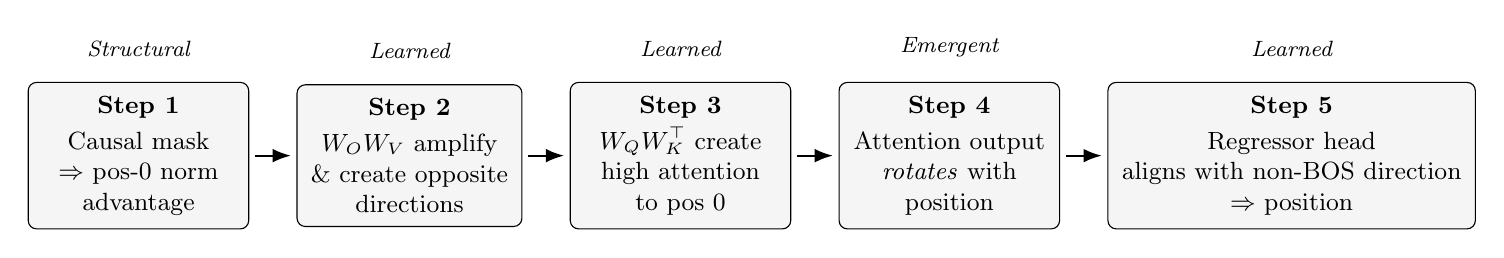
\begin{tikzpicture}[
  font=\small,
  >=Latex,
  node distance=4mm and 6mm,
  stepbox/.style={
    draw, rounded corners=3pt,
    fill=gray!8, align=center,
    inner sep=5pt, minimum width=2.8cm, minimum height=1.8cm
  },
  arr/.style={->, thick, shorten <=2pt, shorten >=2pt}
]

% Step 1
\node[stepbox] (s1) {
  \textbf{Step 1}\\[2pt]
  Causal mask\\
  $\Rightarrow$ pos-0 norm\\
  advantage
};

% Step 2
\node[stepbox, right=of s1] (s2) {
  \textbf{Step 2}\\[2pt]
  $W_OW_V$ amplify\\
  \& create opposite\\
  directions
};

% Step 3
\node[stepbox, right=of s2] (s3) {
  \textbf{Step 3}\\[2pt]
  $W_QW_K^{\top}$ create\\
  high attention\\
  to pos 0
};

% Step 4
\node[stepbox, right=of s3] (s4) {
  \textbf{Step 4}\\[2pt]
  Attention output\\
  \emph{rotates} with\\
  position
};

% Step 5
\node[stepbox, right=of s4] (s5) {
  \textbf{Step 5}\\[2pt]
  Regressor head\\
  aligns with non-BOS direction\\
  $\Rightarrow$ position
};

% Arrows
\draw[arr] (s1) -- (s2);
\draw[arr] (s2) -- (s3);
\draw[arr] (s3) -- (s4);
\draw[arr] (s4) -- (s5);

% Labels
\node[above=2mm of s1, font=\footnotesize\itshape] {Structural};
\node[above=2mm of s2, font=\footnotesize\itshape] {Learned};
\node[above=2mm of s3, font=\footnotesize\itshape] {Learned};
\node[above=2mm of s4, font=\footnotesize\itshape] {Emergent};
\node[above=2mm of s5, font=\footnotesize\itshape] {Learned};

\end{tikzpicture}
\vspace{-1mm}
\caption{\textbf{The geometric gauge mechanism.} Position 0's structural advantage (Step 1) is amplified and converted to opposite directions (Step 2).
Learned attention over-weights position 0 (Step 3), causing the attention output to rotate from the position-0 direction toward the others direction as position increases (Step 4).
A linear head aligned with the others direction reads this rotation (Step 5).}
\label{fig:mechanism_overview}
\end{figure*}

%%%%%%%%%




%%%%%%%%%%%%%%%%%%%%%%%%%%%%%%%%%%%%%%%%%%%%%%%%%%%%%%%%%%%%%%%%%%%%%%%%%%%%%%%
\section{The Mechanism: A Geometric Gauge}
\label{sec:mechanism_text}
%%%%%%%%%%%%%%%%%%%%%%%%%%%%%%%%%%%%%%%%%%%%%%%%%%%%%%%%%%%%%%%%%%%%%%%%%%%%%%%
This section describes the \emph{geometric gauge} mechanism: a circuit that maps a token prefix $(t_0,\dots,t_i)$ in a NoPE Transformer
to an absolute-position estimate $\hat y_i$.
This circuit describes the mechanism by which the Transformer model (described in \ref{sec:notation}) calculates position. We describe a circuit where the weights are randomly initialized, with the exception of the second block's attention and the regression head, which we describe their structure in \Cref{subsec:mechanism}.

Interestingly, we find that while the LayerNorm removes per-position scale, it preserves the \emph{directional} information.
The circuit exploits this by converting a structural, position-dependent \emph{norm asymmetry} (induced by causal prefix averaging in the first attention layer)
into a \emph{directional} positional code.
Concretely, the Block~2 attention write $o_i^{(2)}$ stays within a low-dimensional write subspace and changes its direction smoothly with $i$;
a linear head that projects onto this subspace converts this directional change into $\hat y_i$.
An illustration of this mechanism is displayed in \cref{fig:r0_directional_rotation}.

\subsection{Overview}
\paragraph{Where the position dependence enters.}
The position trace is first created by the causal mask in Block~1: position $0$ (BOS) can only attend to itself, while positions $i>0$ attend to a growing prefix.
This induces a systematic difference in the typical \emph{norm} of the attention aggregation across positions.
Later, Block~2 uses its write operator $B$ together with its attention weights to convert this norm asymmetry into a directionally separable signal.

We call the mechanism a \emph{geometric gauge} because, as position $i$ increases, the direction of the Block~2 attention write $o_i^{(2)}$
moves smoothly within the two-dimensional subspace $\mathrm{span}\{d_{\text{BOS}}, d_{\text{nonBOS}}\}$, from being closer to $d_{\text{BOS}}$
toward being closer to $d_{\text{nonBOS}}$.

In Block~2, the attention write admits the affine form in \Cref{eq:attn_affine_ell} with write operator $B$ defined in \Cref{eq:def_B_ell}.
Using the two unit directions defined in \Cref{sec:notation} (BOS vs.\ non-BOS), the BOS term and the aggregate non-BOS term typically point in different (often opposite) directions.
As the BOS attention weight $\alpha^{(2)}_{i,0}$ decreases with $i$, the direction of $o_i^{(2)}$ shifts from being closer to $d_{\text{BOS}}$ toward being closer to $d_{\text{nonBOS}}$.
A head with nontrivial projection onto $\mathrm{span}\{d_{\text{BOS}},d_{\text{nonBOS}}\}$ converts this directional change into $\hat y_i$.

\subsection{Write map and affine form of the attention update.}
Define the \emph{write map} operator
\begin{equation}
B^{(\ell)} \;:=\; W_O^{(\ell)} W_V^{(\ell)} \in \R^{d\times d}.
\label{eq:def_B_ell}
\end{equation}
Substituting $v_j^{(\ell)} = W_V^{(\ell)}x_j^{(\ell)} + b_V^{(\ell)}$ into $z_i^{(\ell)}$ and then into $o_i^{(\ell)}$ gives
\begin{align}
o_i^{(\ell)}
&= \sum_{j\le i}\alpha_{i,j}^{(\ell)}\, B^{(\ell)} x_j^{(\ell)} \;+\; b_{\text{attn}}^{(\ell)},
\label{eq:attn_affine_ell}
\end{align}
where
\begin{equation}
b_{\text{attn}}^{(\ell)} \;:=\; W_O^{(\ell)} b_V^{(\ell)} + b_O^{(\ell)} \in \R^d.
\end{equation}
Therefore, the attention update to the residual stream can be seen as an affine transformation.

Crucially, since $\sum_{j\le i}\alpha_{i,j}^{(\ell)}=1$ for all $i$, the bias term $b_{\text{attn}}^{(\ell)}$ is constant across positions and cannot by itself encode absolute position.
Accordingly, when analyzing position dependence we focus on $\sum_{j\le i}\alpha_{i,j}^{(\ell)} B^{(\ell)} x_j^{(\ell)}$.

\paragraph{Write-subspace projectors (for interventions).}
Let $B = U\Sigma V^\top$ be the SVD of $B$.
For $r\in\{1,\dots,d\}$, define the projector onto the top-$r$ left-singular subspace:
\begin{equation}
P_r \;:=\; U_{1:r}U_{1:r}^\top.
\end{equation}
We use $P_r$ to retain (or ablate via $I-P_r$) the dominant attention write directions into the residual stream.

\subsection{BOS and non-BOS write directions.}
In Block~2 we summarize the attention-write geometry using two unit directions.
Using the shorthand, define the BOS write vector
\begin{equation}
w_{\text{BOS}} \;:=\; Bx_0 \in \R^d,
\end{equation}
and its normalized direction
\begin{equation}
\label{eq:d_bos}
d_{\text{BOS}} \;:=\; \frac{w_{\text{BOS}}}{\|w_{\text{BOS}}\|} \in \R^d.
\end{equation}
We also define the \emph{non-BOS} write direction as the normalized mean write over positions $j>0$:
\begin{equation}
\label{eq:d_no_bos}
d_{\text{nonBOS}} \;:=\; \frac{\E_{j>0}[Bx_j]}{\|\E_{j>0}[Bx_j]\|} \in \R^d.
\end{equation}

\subsection{A Geometrical Gauge}
\label{subsec:mechanism}

\paragraph{Step 1: Causal inducing a structural norm bias at BOS}
\label{subsec:mech_step1}

Consider Block~1 attention under the causal mask.
Position $0$ can only aggregate information from itself, whereas each position $i>0$ aggregates information from an increasingly long prefix.
When the Block~1 attention distribution is not sharply concentrated on a single token (e.g., it spreads nontrivially over multiple $j\le i$),
the output is an average of multiple token-dependent value vectors.

Averaging multiple vectors typically \emph{reduces} norm unless the vectors are nearly collinear.
Concretely, for any vectors $\{u_j\}$ and nonnegative weights $\{\alpha_j\}$ with $\sum_j \alpha_j = 1$,
\begin{equation}
\Big\|\sum_j \alpha_j u_j\Big\|^2
= \sum_j \alpha_j^2 \|u_j\|^2 \;+\; \sum_{j\neq k} \alpha_j\alpha_k \langle u_j,u_k\rangle.
\label{eq:avg_norm_identity}
\end{equation}
If the mixed vectors are not all aligned (so the cross terms do not all add constructively), then spreading mass over more terms reduces the typical norm.
As the prefix length grows with $i$, this cancellation effect becomes stronger.

Crucially, position $0$ is the unique exception: its prefix contains only itself, so it does not undergo prefix-averaging cancellation.
This creates a \emph{structural} BOS vs.\ non-BOS \emph{norm asymmetry} in Block~1 activations. %it is implied by the causal constraint together with non-peaky attention,
%and does not require any learned positional features.

\paragraph{Step 2: The learned write map amplifies and directionally separates BOS vs.\ non-BOS writes}
\label{subsec:mech_step2}

Step~1 induces a \emph{structural norm bias} in Block~1 $\tilde h_i^{(1)}$ activations: position~0 does not undergo prefix-averaging cancellation, while typical positions $j>0$ do.
Block~2 converts this into a usable \emph{directional} signal via its attention's \textit{write map} operator.
Using the write-map notation from \Cref{eq:def_B_ell,eq:attn_affine_ell}, the Block~2 attention update can be written as
\begin{equation}
o_i^{(2)} \;=\; \sum_{j\le i}\alpha_{i,j}^{(2)}\, B^{(2)} x_j^{(2)} \;+\; b_{\text{attn}}^{(2)}.
\label{eq:mech_step2_attnwrite}
\end{equation}
$o_i^{(2)}$ has the following two characteristics:
\setlength{\parskip}{0pt}

\paragraph{(i) Position asymmetry amplification.}
The BOS write vector $w_{\text{BOS}}:=B^{(2)}x_0^{(2)}$ typically has larger norm than a typical non-BOS write $B^{(2)}x_j^{(2)}$ for $j>0$ (equivalently, $\|w_{\text{BOS}}\|$ is large relative to the aggregate non-BOS write).
This matters because the attention write is added into the residual stream before subsequent normalization:
a larger-norm component in the sum $h_i^1 + o_i^{(2)}$ more strongly determines the \emph{direction} of that sum.
LayerNorm rescales (after centering) but does not undo which component dominates the direction, so this directional tilt can persist to later computations.
\setlength{\parskip}{0pt}
\paragraph{(ii) Directional separation.}
Beyond amplification, $B^{(2)}$ maps the BOS input and typical non-BOS inputs to \emph{well-separated directions}.
Concretely, $w_{\text{BOS}}$ aligns with $d_{\text{BOS}}$, while the non-BOS writes $\{B^{(2)}x_j^{(2)}\}_{j>0}$ are approximately aligned with $d_{\text{nonBOS}}$ (definitions in \Cref{sec:notation}).
As a result, the position-dependent attention weights $\alpha_{i,j}^{(2)}$ control a mixture between two stable write directions,
so $o_i^{(2)}$ lies approximately in the plane $\mathrm{span}\{d_{\text{BOS}}, d_{\text{nonBOS}}\}$.
This sets up Step~3, where learning in $W_Q^{(2)},W_K^{(2)}$ makes the BOS weight $\alpha_{i,0}^{(2)}$ vary with $i$.

\paragraph{Step 3: Learned queries/keys create a position-dependent BOS attention mass}
\label{subsec:mech_step3}

Step~2 establishes two stable write directions (definitions in \Cref{sec:notation}): $d_{\text{BOS}}$ and $d_{\text{nonBOS}}$.
Step~3 supplies the \emph{position-dependent scalar} that mixes these directions: the BOS attention mass $\alpha_{i,0}^{(2)}$.

\paragraph{BOS is made unusually salient as a key.}
The learned query/key projections $W_Q^{(2)},W_K^{(2)}$ make the BOS key $k_0^{(2)}$ score salient for queries $q_i^{(2)}$ compared to $k_{j>0}^{(2)}$.
Equivalently, the BOS logit $s_{i,0}^{(2)}$ is typically larger than $s_{i,j}^{(2)}$ for many $j>0$.
Consequently, $\alpha_{i,0}^{(2)}$ is large compared to a typical non-BOS weight, so the write term
$\sum_{j\le i}\alpha_{i,j}^{(2)} B^{(2)}x_j^{(2)}$ places substantial weight on the BOS write $B^{(2)}x_0^{(2)}$.
For small $i$, this makes the Block~2 write direction closer to $d_{\text{BOS}}$.

\paragraph{Why $\alpha_{i,0}^{(2)}$ decreases with position.}
Due to the causal mask, at query position $i$ the softmax normalizes only over keys in the prefix $j\le i$.
As $i$ increases, the number of competing non-BOS keys grows, increasing the softmax normalizer.
Unless the BOS logit advantage $s_{i,0}^{(2)}$ grows with $i$ strongly enough to offset this expanding competition,
the BOS attention mass $\alpha_{i,0}^{(2)}$ decreases with $i$.
This provides the monotone position dependence used in Step~4.

\paragraph{Step 4: The Block~2 attention write rotates between the two directions}
\label{subsec:mech_step4}

Combine Steps~2--3. The Block~2 attention update is a convex combination of the written vectors $\{B x_j\}_{j\le i}$.
Under concentration of the non-BOS aggregate around $w_{\text{other}}$, the update is well-approximated by a two-direction
mixture:
\begin{equation}
o_i^{(2)}
\;\approx\;
\alpha_{i,0}^{(2)}\, w_0
\;+\;
\big(1-\alpha_{i,0}^{(2)}\big)\, w_{\text{other}}
\;+\;
b_{\text{attn}}^{(2)}.
\label{eq:two_dir_mixture_mech}
\end{equation}
As $i$ increases, $\alpha_{i,0}^{(2)}$ decreases, so $o_i^{(2)}$ moves continuously from the BOS direction toward the
others direction. Geometrically, this is a smooth trajectory (``rotation'') in the plane spanned by
$\{w_0,w_{\text{other}}\}$.
This effect is exemplified in \Cref{fig:r0_gauge}.

\paragraph{Step 5: Reading the rotation from the residual stream}
\label{subsec:mech_step5}

The final residual stream after Block~2 is
\begin{equation}
h_i^2 \;=\; h_i^1 + o_i^{(2)} + \MLP_2\!\Big(\LN(h_i^1 + o_i^{(2)})\Big),
\end{equation}
and the model predicts position by
\begin{equation}
\hat y_i \;=\; w_{\text{head}}^\top h_i^2 + b_{\text{head}}.
\end{equation}
Because $b_{\text{attn}}^{(2)}$ is constant in $i$, it can be absorbed into $b_{\text{head}}$ and does not affect the
position-dependent part of the readout.
The mechanism requires that $w_{\text{head}}$ has nontrivial projection onto the geometric-gauge plane
$\mathrm{span}\{w_0,w_{\text{other}}\}$, so that $w_{\text{head}}^\top h_i^2$ varies monotonically with the mixing
coefficient $\alpha_{i,0}^{(2)}$.
In other words, the head converts the \emph{directional rotation} produced by Block~2 into a scalar position estimate.

\subsection{Position signal survives the LayerNorm}
\label{subsec:mech_implications}

LayerNorm removes per-sample magnitude, ruling out any mechanism that depends purely on norm/variance at a single position. The geometric gauge avoids this by representing position in \emph{direction}: learning uses the write map $B$ to create two
stable poles ($w_0$ and $w_{\text{other}}$), and attention causal mask supplies a position-dependent mixture coefficient
$\alpha_{i,0}^{(2)}$ that modulates direction rather than scale.

%%%%%%%%%%%%%%%%%%%%%%%%%%%%%%%%%%%%%%%%%%%%%%%%%%%%%%%%%%%%%%%%%%%%%%%%%%%%%%%
\section{Empirical Evidence}
\label{sec:empirical}
%%%%%%%%%%%%%%%%%%%%%%%%%%%%%%%%%%%%%%%%%%%%%%%%%%%%%%%%%%%%%%%%%%%%%%%%%%%%%%%

We validate the geometric gauge mechanism in two complementary regimes.
First, in \Cref{subsec:minimal_evidence}, we study \modelminimal: a controlled two-block NoPE Transformer in which only Block~2's attention (single head) and the linear position head are trained, while all other components are frozen at random initialization.
This isolates the circuit and enables direct, step-by-step measurements.
Second, in \Cref{subsec:full_evidence}, we analyze \modelfull: a fully trained two-block Transformer with 12 attention heads per block.
Interestingly, despite greater capacity, \modelfull converges to the same BOS-anchored, two-direction geometry, demonstrating that the mechanism is learnable using gradient-based optimization in NoPE architectures.

\subsection{Experimental Setup}
\paragraph{Data and splits.}
We train and evaluate on sequences from OpenWebText \citep{} with a BOS token prepended.
Training uses disjoint text sequences from validation; the target is absolute position $i\in\{0,\dots,L{-}1\}$ within each sequence.
Unless stated otherwise, models are trained at length $L=128$ and evaluated on held-out validation sequences at the same length.

\paragraph{Metric.}
We report coefficient of determination $R^2$ between predictions $\hat y_i$ and true positions $i$ over all tokens in the evaluated set.
% For length extrapolation curves, we additionally report squared Pearson correlation ($r^2$) between $\hat y_i$ and $i$ to factor out global affine rescaling.

\paragraph{Reporting convention.}
Unless stated otherwise, scalar summaries in this section are computed on the same fixed validation batch of $n_{\text{seq}}=64$ sequences (yielding 8,192 evaluated tokens).

\paragraph{Models \& Training.}
% We evaluate on OpenWebText with BOS prepended and training length $L=128$.
We have two models variants, both include a 2-block pre-norm Transformer ($d=768$, no positional embeddings) 
initialized with Xavier initialization \citep{glorot2010understanding}.
\modelminimal has a single attention head in both blocks, and most of its weights are frozen besides the second block's attention, and the regression head.
% and Block~2 trains attention plus a linear position head; the Block~2 MLP and LayerNorm are frozen, and the head reads the full Block~2 output.
\modelfull include 12 heads per block, and trains all parameters.
\modelminimal is trained for 40K steps and \modelfull for 20K steps. 
We report best-checkpoint metrics for all models based on the regression validation MSE loss.

%%%%%%%%%%%%%%%%%%%%%%%%%%%%%%%%%%%%%%%%%%%%%%%%%%%%%%%%%%%%%%%%%%%%%%%%%%%%%%%
\subsection{\modelminimal: Validating the Mechanism in a Controlled Setting}
\label{subsec:minimal_evidence}
%%%%%%%%%%%%%%%%%%%%%%%%%%%%%%%%%%%%%%%%%%%%%%%%%%%%%%%%%%%%%%%%%%%%%%%%%%%%%%%

\modelminimal achieves strong position decoding with a single trainable attention head in Block~2: $R^2=0.990$ (evaluated on $n=640$ sequences).
We now quantify each step of the geometric gauge.

\paragraph{Step 1: Causal prefix averaging creates a BOS norm advantage.}
With Block~1 frozen with random initialization, its attention weights remain near-uniform over the causal prefix (see \Cref{fig:attn_maps_empirical}, left).
We quantify the uniformity of this randomly initialized attention weight using average entropy per query position, as each query defines a probability distribution over keys.
The mean entropy is 3.77, compared to a perfectly uniform attention has \(\frac{1}{128}\sum_{t=0}^{127}\log(t+1) = 3.878\), and an attention weight concentrated at one position with 0 mean entropy.
This uniform attention head then got multiplied by the value vectors, yielding an increasing uniform prefix-averaging value vectors.
Therefore, positions $i>0$ undergo prefix-averaging cancellation while position~0 (BOS) cannot average with any other token because of the causal mask.
Empirically, Block~1 attention outputs exhibit a larger BOS norm compared to non-BOS tokens:
\[
\|o^{(1)}_{\text{BOS}}\|=10.5
\quad\text{vs.}\quad
\E_{\text{nonBOS}}\!\left[\|o^{(1)}_j\|\right]=2.27
\quad (4.64\times).
\]
The norm asymmetry is \emph{structural}: it follows the causal transformer together with non-peaky attention weights.


\paragraph{Step 2: Learned write map amplifies and separates BOS vs.\ non-BOS writes.}
Block~2 converts the structural norm bias into a directional form via the write map $B=W_O W_V$.
In \Cref{eq:mech_step2_attnwrite}, the multiplication by $B$ strongly amplify BOS's norm and map BOS and non-BOS to opposite directions, defined by $d_{\text{BOS}}$ \eqref{eq:d_bos} and $d_{\text{nonBOS}}$ \eqref{eq:d_no_bos} respectively.
Hence, the scalar products are:
\[
\|W_O v_{\text{BOS}}\|=394.9
\quad\text{vs.}\quad
\|W_O v_{\text{nonBOS}}\|=89.8
\quad (4.40\times),
\]
and the empirical BOS and non-BOS directions are anti-correlated,
\[
\cos(d_{\text{BOS}}, d_{\text{nonBOS}})=-0.660.
\]
This directional separation sets up a two-pole geometry in which attention can encode position via a mixing coefficient.

\paragraph{Step 3: Learned attention over-weights BOS.}
Block~2 query/key projections make $\text{BOS}$ salient as a key, producing a large $\text{BOS}$ attention mass.
At query position $i=50$, the mean $\text{BOS}$ weight is
\[
\alpha^{(2)}_{50,\text{BOS}}=0.329
\quad\text{vs.}\quad
1/51=0.0196 \text{ (uniform)},
\]
corresponding to a $16.8\times$ over-weighting.
Thus, early in the sequence the Block~2 attention update contains a substantial $\text{BOS}$ contribution.

To quantify $\text{BOS}$ preference at the \emph{head} level, \Cref{tab:block2_bos_ratio} reports a $\text{BOS}$-bias ratio for each head $h$.
Let $a^{(2)}_{b,h}(t,j)$ denote the attention weight in Block~2, head $h$, for sequence $b$, query position $t$, and key position $j$.
We use the shorthand $a^{(2)}_{b,h}(t,\text{BOS}) \defeq a^{(2)}_{b,h}(t,0)$ and define
\begin{align}
\label{eq:bos_attendence_metric}
&r_h \;:=\;
\frac{\E_{b,\,t\ge0}\!\big[a^{(2)}_{b,h}(t,\text{BOS})\big]}
{\E_{b,\,t>0}\!\big[\;\overline{a}^{(2)}_{b,h}(t,\text{nonBOS})\big]},
\\
&\overline{a}^{(2)}_{b,h}(t,\text{nonBOS}) \;:=\; \frac{1}{t}\sum_{j=1}^{t} a^{(2)}_{b,h}(t,j).
\end{align}

That is, $r_h$ is the average attention mass assigned to $\text{BOS}$ divided by the average mass assigned to a $\text{nonBOS}$ key.
In \modelminimal, the learned Block~2 head exhibits $\approx 22\times$ $\text{BOS}$ bias.
In \modelfull, multiple heads show strong $\text{BOS}$ preference—often with substantially larger ratios—indicating that $\text{BOS}$ salience emerges robustly under full training.



\paragraph{Step 4: Attention output rotates between two stable directions.}
As the effective BOS mass varies with position, the Block~2 attention output traces a smooth trajectory in the plane spanned by the BOS and others directions.
Quantitatively, directional projections correlate strongly and with opposite signs:
\begin{align*}
&\mathrm{Spearman}(o_t\!\cdot\! d_{\text{BOS}},\, t)=-1,\\
&\mathrm{Spearman}(o_t\!\cdot\! d_{\text{nonBOS}},\, t)=+1,
\end{align*}

visualized in \Cref{fig:r0_gauge}.

\paragraph{Step 5: Linear head reads the rotation.}
The learned head aligns with the others direction, consistent with reading out the BOS-to-others rotation:
\[
\cos(w_{\text{head}}, d_{\text{nonBOS}})=0.731.
\]
Together, Steps 2--5 convert the causal BOS advantage into a directional form that is linearly readable at the output.
Strikingly, the linear head aligns with $d_{\text{nonBOS}}$, which represents allows extracting the position as the angle between

\textbf{\modelfull.} The head also aligns with the others direction ($\cos=0.319$, $n=64$) and achieves $R^2=0.997$ on $n=640$ sequences.

\begin{figure}[t]
\centering
\begin{subfigure}{0.49\columnwidth}
\centering
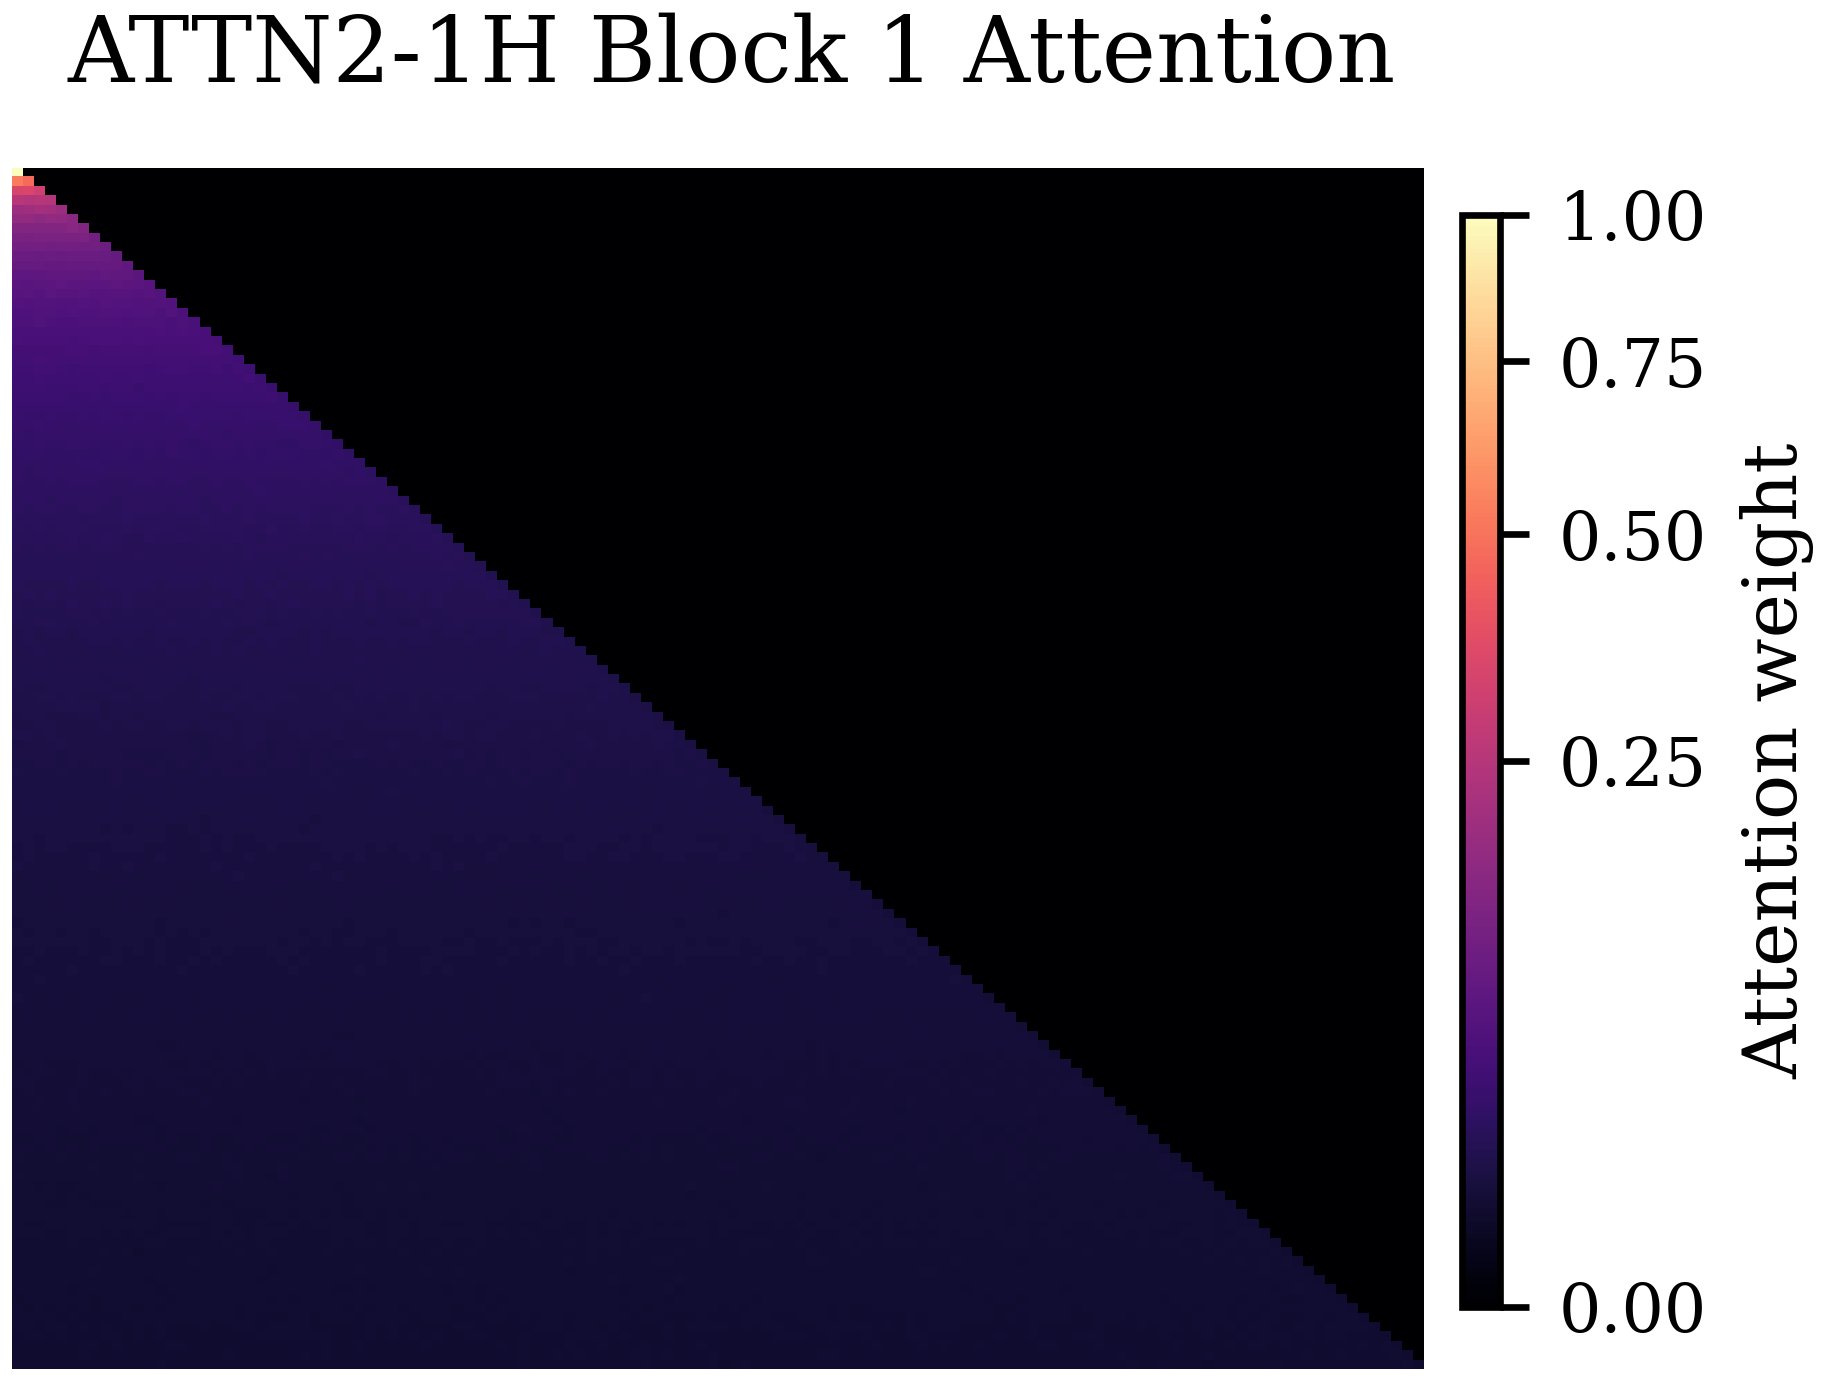
\includegraphics[width=\linewidth]{plots/attention_uniformity/attn2_1h_block1_attention.png}
\caption{\modelminimal 1st block attention map.}
\end{subfigure}
\begin{subfigure}{0.49\columnwidth}
\centering
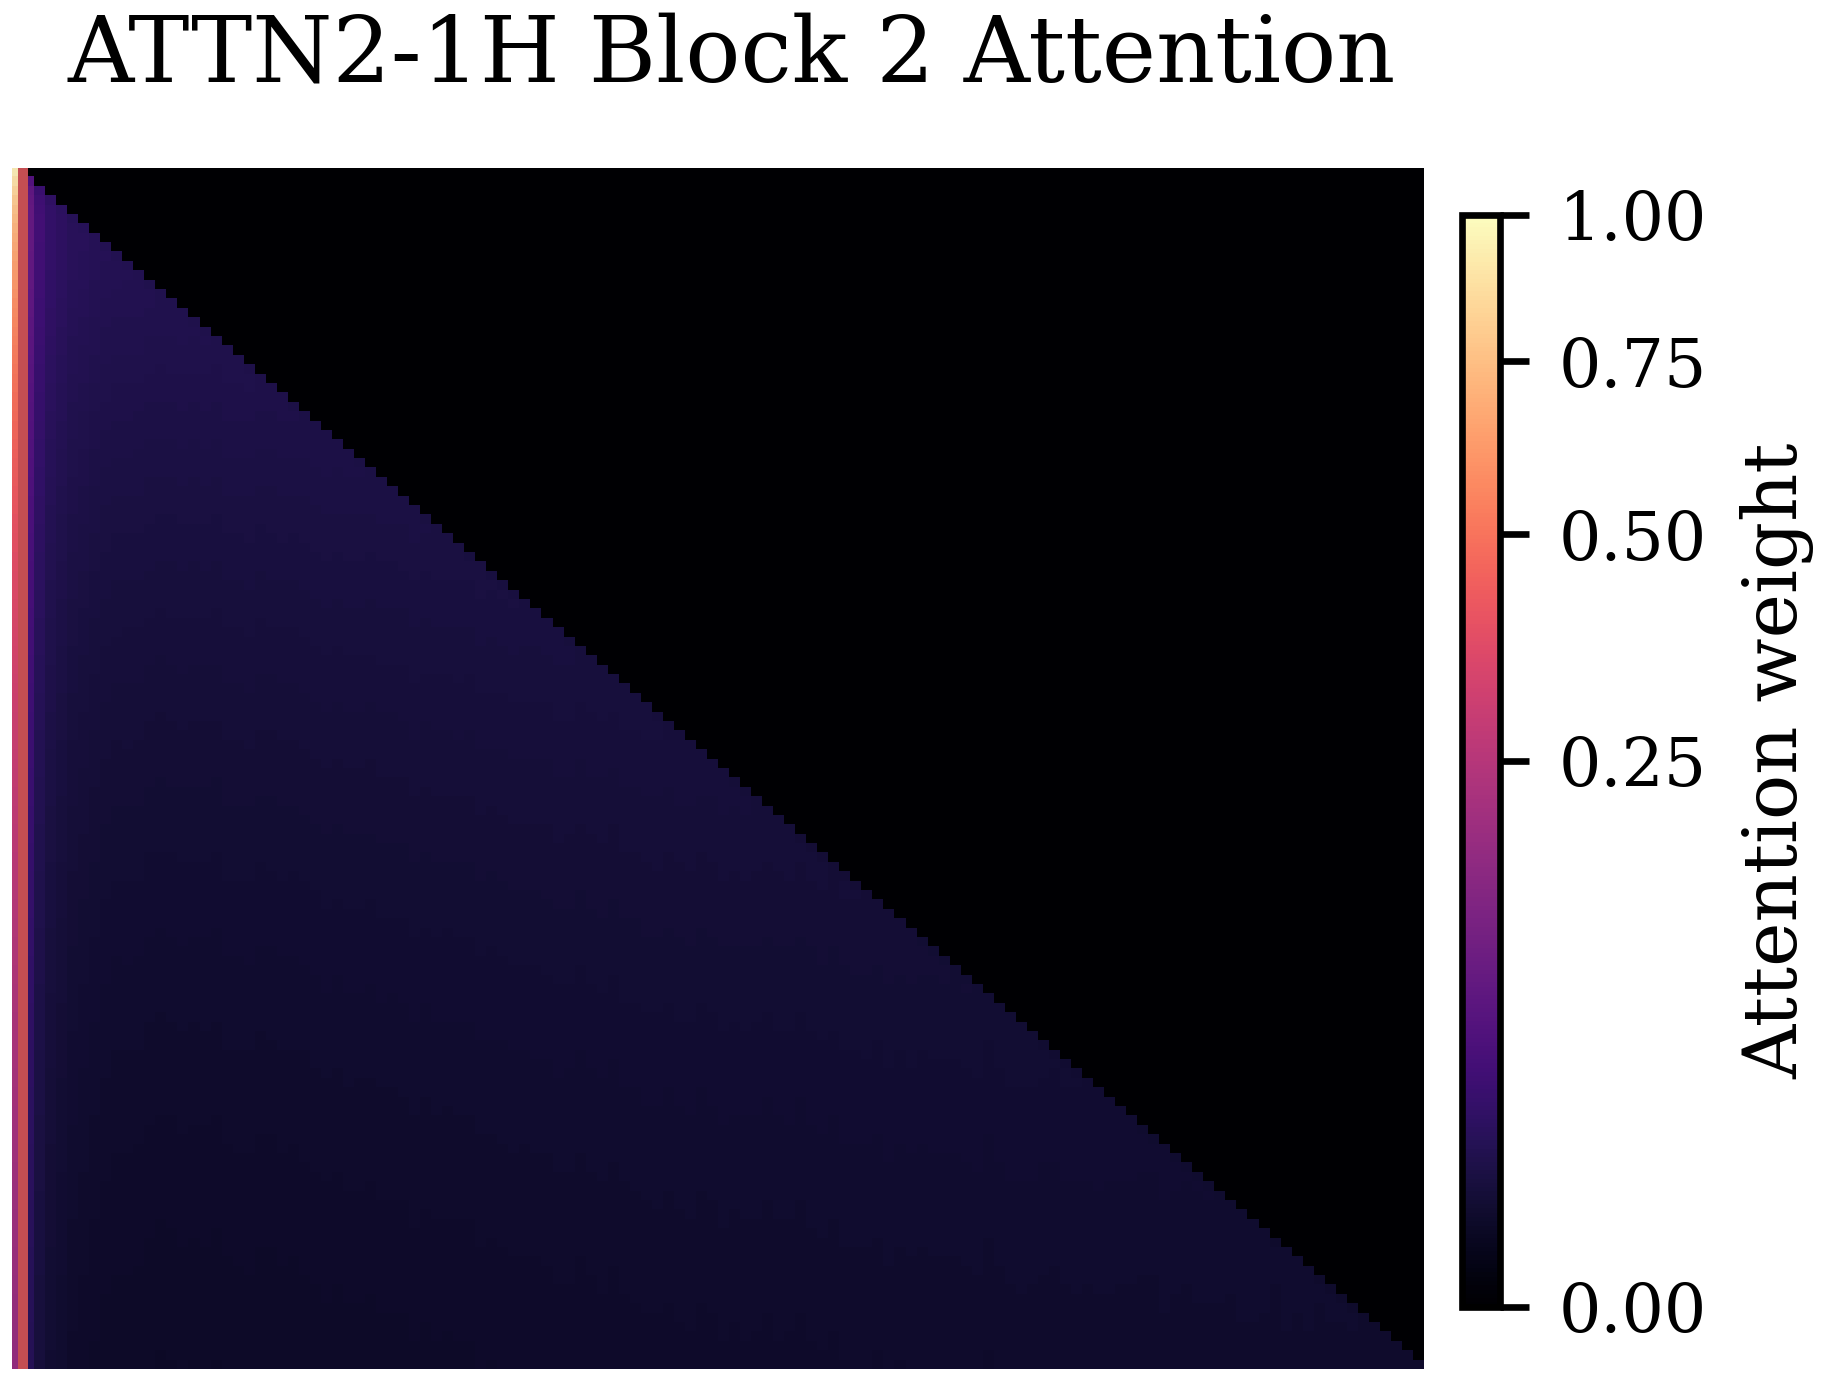
\includegraphics[width=\linewidth]{plots/attention_uniformity/attn2_1h_block2_attention.png}
\caption{\modelminimal 2nd block attention map.}
% , BOS-attending ratio is $~22\times$.}
\end{subfigure}
\caption{\modelminimal \textbf{Attention maps.} Xavier initialization with inductive bias induce Block~1 almost-uniform attention weights at initialization, where Block~2 (learned) concentrates on BOS. Its quantified BOS-attendance is $r_h\approx22$ \eqref{eq:bos_attendence_metric}. }
\label{fig:attn_maps_empirical}
\vspace{-2mm}
\end{figure}

\begin{figure}[t]
\centering
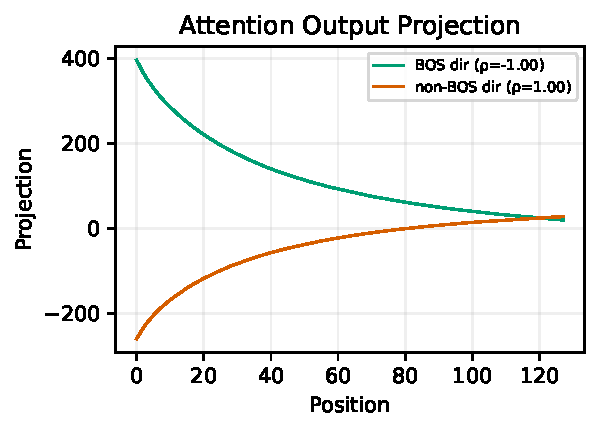
\includegraphics[width=\columnwidth]{plots/r0_attention_output_projection/attention_output_projection_attn2_1h.pdf}
\caption{\textbf{Geometric gauge projections (\modelminimal).}
$o_t^2$ scalar product with $d_{\text{BOS}}$ and $d_{\text{nonBOS}}$}
\label{app:geom_gauge_fullblock}
\vspace{-2mm}
\end{figure}
\begin{figure}[t]
\centering
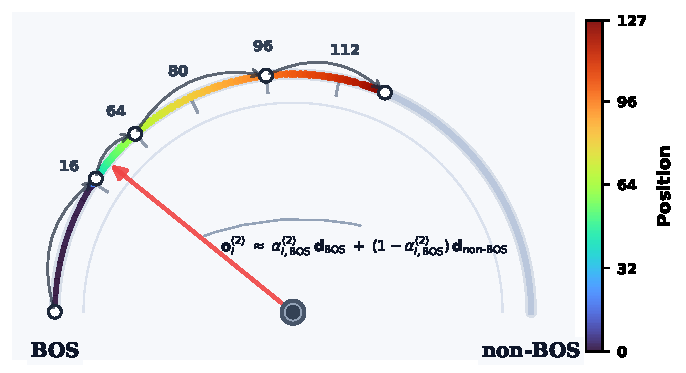
\includegraphics[width=\columnwidth]{r0_directional_rotation_example.pdf}
\caption{\textbf{Directional rotation gauge (\modelfull, averaged).}}
Average gauge trajectory over $n=64$ sequences; markers every 16 positions.
\label{fig:r0_gauge}
\vspace{-2mm}
\end{figure}
%%%%%%%%%%%%%%%%%%%%%%%%%%%%%%%%%%%%%%%%%%%%%%%%%%%%%%%%%%%%%%%%%%%%%%%%%%%%%%%
\subsection{\modelfull: Convergence to the Geometric Gauge Under Full Training}
\label{subsec:full_evidence}
%%%%%%%%%%%%%%%%%%%%%%%%%%%%%%%%%%%%%%%%%%%%%%%%%%%%%%%%%%%%%%%%%%%%%%%%%%%%%%%

\modelfull attains near-perfect position decoding ($R^2=0.997$ on $n=640$ sequences) and exhibits the same BOS-anchored two-direction geometry as \modelminimal.
Rather than repeating the step-by-step analysis, we highlight the \emph{differences} that arise under full training and use the gauge visualization (\Cref{fig:r0_gauge}) as the main summary.
Complete quantitative diagnostics for Steps~1--5 (per-head statistics, attention maps, and projection curves) appear in \Cref{app:full_evidence_app}.

\paragraph{Same qualitative mechanism, with stronger two-pole geometry.}
Under full training, the effective write subspace is still well-approximated by two stable poles aligned with
$d_{\text{BOS}}$ and $d_{\text{nonBOS}}$, but the separation is cleaner than in \modelminimal
(e.g., $\cos(d_{\text{BOS}},d_{\text{nonBOS}})\approx -0.97$; see \Cref{app:geom_gauge_fullblock}).
This sharper two-pole structure makes the downstream rotation easier to visualize and measure.

\paragraph{Multiple heads implement BOS salience.}
Unlike \modelminimal (single trained head), \modelfull distributes the BOS preference across several Block~2 heads.
We report the per-head BOS-bias ratios $r_h$ in \Cref{tab:block2_bos_ratio}; several heads strongly over-attend to BOS,
while others do not, indicating a heterogeneous but robust implementation.

\paragraph{Gauge visualization: smooth BOS-to-others rotation across positions.}
To summarize the mechanism in \modelfull, we visualize the Block~2 attention write direction as a \emph{gauge} between
$d_{\text{BOS}}$ and $d_{\text{nonBOS}}$ (\Cref{fig:r0_gauge}).
As position increases, the gauge angle advances smoothly from the BOS pole toward the non-BOS pole, consistent with a
monotone decrease in the BOS mixture coefficient $\alpha^{(2)}_{i,0}$.
Per-sequence gauges (showing the effect holds at the individual-sequence level) are provided in \Cref{app:gauge_grid}.

\paragraph{Readout differs: weaker head alignment due to additional pathways.}
The regression head remains aligned with the non-BOS pole but less strongly than in \modelminimal
(e.g., $\cos(w_{\text{head}},d_{\text{nonBOS}})\approx 0.32$).
A natural explanation is that, in \modelfull, the trained Block~2 MLP can also contribute position information, so the
linear head need not rely as directly on the pure attention-rotation signal.

\paragraph{Takeaway.}
Despite full parameter freedom and multi-head capacity, \modelfull converges to the same BOS-anchored geometric gauge
identified in \modelminimal; the gauge in \Cref{fig:r0_gauge} provides a compact main-text summary, with full step-wise
measurements deferred to \Cref{app:full_evidence_app}.


%%%%%%%%%%%%%%%%%%%%%%%%%%%%%%%%%%%%%%%%%%%%%%%%%%%%%%%%%%%%%%%%%%%%%%%%%%%%%%%
\section{Write Bottleneck: Validating the Mechanism}
\label{sec:write_bottleneck}
%%%%%%%%%%%%%%%%%%%%%%%%%%%%%%%%%%%%%%%%%%%%%%%%%%%%%%%%%%%%%%%%%%%%%%%%%%%%%%%
To validate that position information flows through a low-dimensional write subspace,
we perform a causal intervention on the Block~2 attention update.
\paragraph{Write-subspace intervention.}
Let $B = U\Sigma V^\top$ be the SVD decomposition of the write map.
We define the rank-$r$ projector as $P_r := U_{1:r}U_{1:r}^\top$.
We define two intervention mechanisms directly on the Block~2 attention update $o_i$, named \textit{retention} and \textit{ablation}:
\begin{align}
\tilde o_i &:= P_r\, o_i \quad \text{(retain top-$r$ directions)} \\
\tilde o_i &:= (I-P_r)\, o_i \quad \text{(ablate top-$r$ directions)}.
\end{align}
Retention \textit{keeps} the top-$r$ directions of the write map, while ablation \textit{removes} the top-$r$ directions.
\paragraph{Intervened forward pass.}
We replace the attention update in the Block~2 residual stream:
\begin{align}
\tilde h_i^{(2)} &:= h_i^{1} + \tilde o_i,
\end{align}
All other computations (LayerNorms, MLP, and the position head) are unchanged.
We evaluate $R^2$ between predicted and true positions on $n=1600$ sequences.
\begin{figure*}[t]
\centering
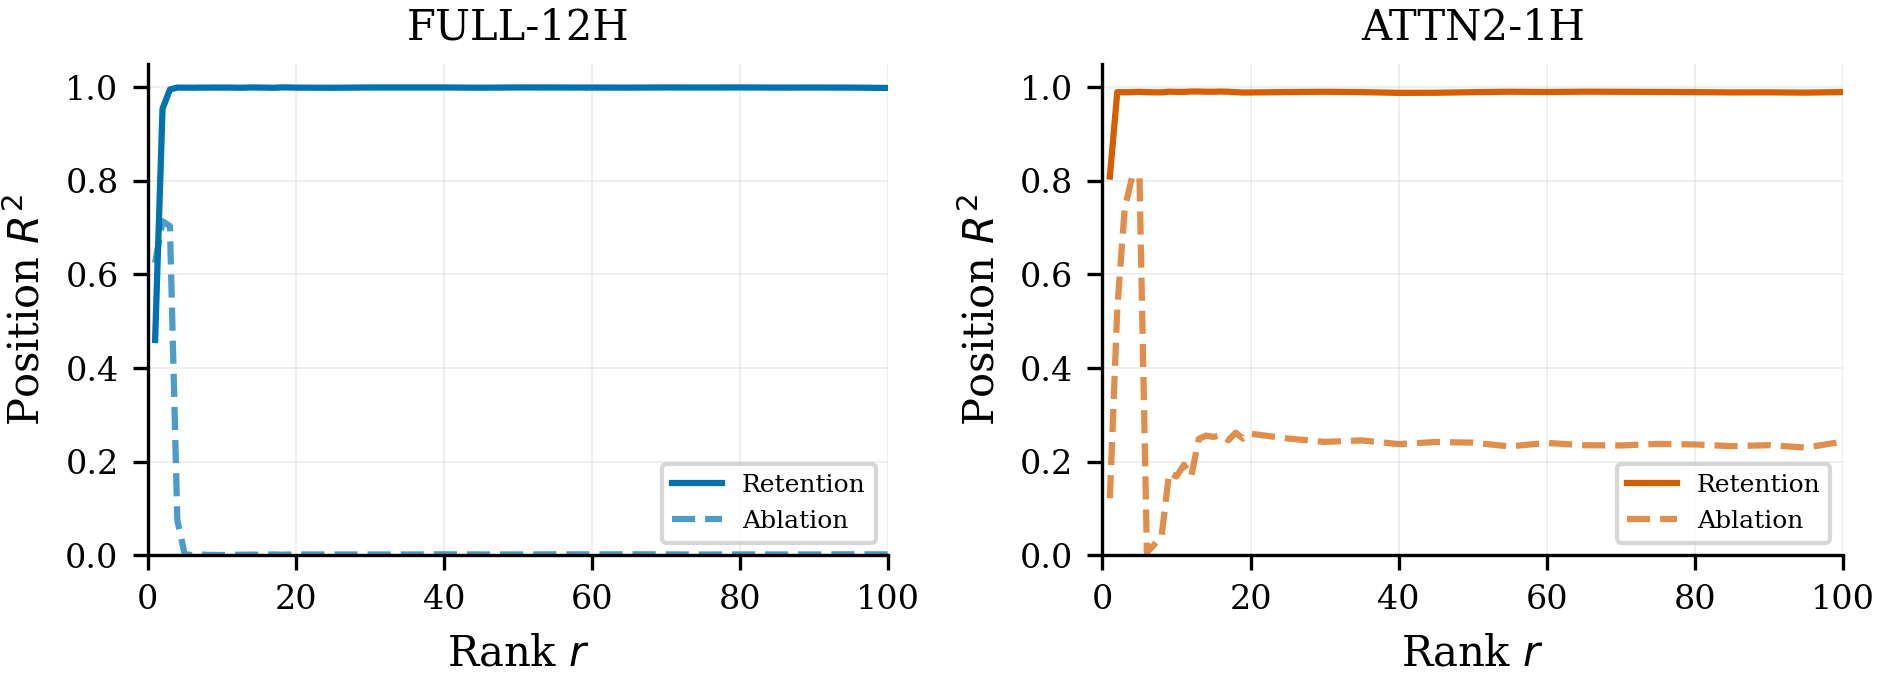
\includegraphics[width=0.95\textwidth]{plots/write_bottleneck_curves_all.png}
\caption{\textbf{Write bottleneck.}
Position decoding is recovered with only two singular vectors of the write map $B$.
Both \modelminimal (ATTN2-1H) and \modelfull (FULL-12H) exhibit a low-rank bottleneck.}
\label{fig:write_bottleneck}
\vspace{-2mm}
\end{figure*}
Intervention results presented in \Cref{fig:write_bottleneck}.

\paragraph{Results: \modelminimal.}
The correlation between the predicted and true positions without our intervention is $R^2=0.990$.
Retention of the top-1 singular direction yields $R^2=0.809$,
while top-2 retention recovers $R^2=0.990$, recovering the same correlation before the intervention.
When ablating the top-1 direction, the correlation drops to $R^2=0.131$.
Taken together, these results indicate that two directions of the \textit{write map} account are responsible for tracking the position of sequences in our NoPE transformer models.
\paragraph{Results: \modelfull.}
We observe similar trends with the second model.
While the non-intervened model's correlation is $R^2=0.9999$, 
retaining the top-1 and top-2 singular directions yields $R^2=0.460$ and $R^2=0.953$, respectively.
Top-1 ablation drops performance to $R^2=0.624$

% \section{Conclusions}

%%%%%%%%%%%%%%%%%%%%%%%%%%%%%%%%%%%%%%%%%%%%%%%%%%%%%%%%%%%%%%%%%%%%%%%%%%%%%%%
\section{Conclusions}
%%%%%%%%%%%%%%%%%%%%%%%%%%%%%%%%%%%%%%%%%%%%%%%%%%%%%%%%%%%%%%%%%%%%%%%%%%%%%%%

% \paragraph{A complete mechanism.}
The geometric gauge provides a complete account of position encoding in NoPE Transformers:
structural availability (causal mask), learned extraction (directional separation), and learned readout (aligned head).
Using two experiments of a simple transformer model that they both converge into the proposed mechanism of the geometric gauge, suggesting it is a natural mechanism for models to learn through gradient decent.
The low rank of the attention head $r_{95}=2$ confirms that position flows through a minimal subspace---the plane spanned by position-0 and others directions.
% The fully trained R0 model converges to this same mechanism despite having the freedom to learn any position-encoding strategy, suggesting the geometric gauge is a natural attractor of gradient-based optimization in NoPE architectures.

% \paragraph{Reconciling with prior work.}
While \citet{chi-etal-2023-latent} identified that causal attention creates position-dependent variance, an open question remained on how the position information can survive the layer norm.
We show that LayerNorm, while removing the magnitude signal, keeps a directional signal, and the geometric gauge is the mechanism that makes it linearly readable.

% \paragraph{The write bottleneck.}
% The extremely low $r_{95}=2$ for the 1-head model confirms that position flows through a minimal subspace---the plane spanned by position-0 and others directions.


%%%%%%%%%%%%%%%%%%%%%%%%%%%%%%%%%%%%%%%%%%%%%%%%%%%%%%%%%%%%%%%%%%%%%%%%%%%%%%%
\section*{Impact Statement}
%%%%%%%%%%%%%%%%%%%%%%%%%%%%%%%%%%%%%%%%%%%%%%%%%%%%%%%%%%%%%%%%%%%%%%%%%%%%%%%
This work studies mechanistic understanding of positional information in transformer models. No direct negative
societal impacts are anticipated.

\bibliography{custom}
\bibliographystyle{icml2025}

\clearpage

%%%%%%%%%%%%%%%%%%%%%%%%%%%%%%%%%%%%%%%%%%%%%%%%%%%%%%%%%%%%%%%%%%%%%%%%%%%%%%%
\appendix
%%%%%%%%%%%%%%%%%%%%%%%%%%%%%%%%%%%%%%%%%%%%%%%%%%%%%%%%%%%%%%%%%%%%%%%%%%%%%%%

\section{Additional Experimental Details}
\label{app:details}

\paragraph{Training.}
AdamW optimizer, learning rate $6\times10^{-4}$ with cosine decay, 20K steps.
Batch size 64, gradient accumulation 2.


%%%%%%%%%%%%%%%%%%%%%%%%%%%%%%%%%%%%%%%%%%%%%%%%%%%%%%%%%%%%%%%%%%%%%%%%%%%%%%%
\section{\modelfull: Convergence to the Geometric Gauge Under Full Training}
\label{app:full_evidence_app}
%%%%%%%%%%%%%%%%%%%%%%%%%%%%%%%%%%%%%%%%%%%%%%%%%%%%%%%%%%%%%%%%%%%%%%%%%%%%%%%

\modelfull achieves high position decoding despite full parameter freedom: $R^2=0.997$ (evaluated on $n=640$ sequences).
We find the same step-by-step signatures of the geometric gauge.

\paragraph{Step 1: Block~1 preserves causal prefix averaging.}
Although Block~1 is fully trainable in \modelfull, it retains a similar causal prefix-averaging pattern observed in \modelminimal (\Cref{fig:full12h_block1_attention}, up).
Consistent with prefix averaging, the Block~1 attention write exhibits a clear BOS norm advantage.
For example, for heads 8 and 10 we find
\begin{align*}
&|o^{(1,8)}_t(x_{\text{BOS}})\| \in [3.941,\,3.921]
\quad\text{vs.}\\
&|o^{(1,10)}_t(x_{\text{nonBOS}})\| \in [0.785,\,0.812],
\end{align*}
corresponding to an approximate $5.0\times$ norm ratio.
This advantage of the norm ratio for BOS aligns with \modelminimal.

\paragraph{Step 2: Stronger directional separation under full training.}
Aggregating across all heads (fused $B=W_O W_V$), the BOS/non-BOS separation is even cleaner:
\[
\|W_O v_{\text{BOS}}\|=1847.7
\quad\text{vs.}\quad
\|W_O v_{\text{others}}\|=743.4
\quad (2.49\times),
\]
with near-perfect anti-correlation between directions,
\[
\cos(d_{\text{BOS}}, d_{\text{nonBOS}})=-0.969
\]
Equivalently, the angle between $d_{\text{BOS}}$ and $d_{\text{nonBOS}}$ is close to $180^\circ$, indicating that full training yields a more pronounced two-pole geometry in the write subspace.
One possible interpretation is that increasing the separation between these directions makes the subsequent rotation in $\mathrm{span}\{d_{\text{BOS}}, d_{\text{nonBOS}}\}$ easier to read out.

\paragraph{Step 3: Multiple heads over-weight BOS.}
At $i=50$, mean BOS attention is $\alpha_{50,0}=0.290$ (uniform $1/51=0.0196$), an over-weighting of $14.8\times$ ($n=64$).
This indicates that BOS salience emerges robustly across heads.

\begin{table}[H]
\centering
\small
\caption{\textbf{Block~2 $\text{BOS}$-bias ratio per head.}
For each head $h$, we compute the BOS-attendence metric in \cref{eq:bos_attendence_metric}
on BOS-prepended OpenWebText validation sequences, averaged over 1280 sequences.}
\label{tab:block2_bos_ratio}
\setlength{\tabcolsep}{3pt}
\resizebox{\columnwidth}{!}{
\begin{tabular}{l cccccccccccc}
\toprule
Model & H0 & H1 & H2 & H3 & H4 & H5 & H6 & H7 & H8 & H9 & H10 & H11 \\
\midrule
ATTN2-1H & 21.900 & -- & -- & -- & -- & -- & -- & -- & -- & -- & -- & -- \\
FULL-12H & 0.369 & \textbf{15.472} & $7.22\times10^{-18}$ & \textbf{11.200} & \textbf{36.013} & \textbf{76.720} & 0.029 & \textbf{101.295} & \textbf{3.026} & \textbf{26.638} & \textbf{33.347} & \textbf{62.871} \\
\bottomrule
\end{tabular}}
\vspace{-2mm}
\end{table}

\paragraph{Step 4: A gauge visualization shows smooth BOS-to-others rotation.}
We analyze the Block‑2 attention update \(o_i^{(2)}\) within the write map \(B^{(2)}\). We remove the affine bias term in \eqref{eq:attn_affine_ell} and project the resulting attention write onto the two unit directions \(d_{\text{BOS}}\) and \(d_{\text{nonBOS}}\) (\eqref{eq:d_bos}, \eqref{eq:d_no_bos}). The gauge angle at each position \(i\) is the normalized angular position of \(o_i^{(2)}\) between these directions. For the individual (averaged‑base) plot, average \(o_i^{(2)}\) across the batch at each \(i\). ~\Cref{fig:r0_gauge} shows the resulting gauge trajectory over \(i=0,\dots,n-1\) (a subset). Moreover, we repeat the same computation per sequence (no cross‑sequence averaging) and visualize 12 independent sequences in \cref{app:gauge_grid}, presenting the geometry of 12 random sequences, aimed to demonstrate how the mechanism operates at the \emph{individual sequence} level.
The arrows in the gauge indicate the temporal progression between consecutive positions in the graph.
We also measured quantitavly this geometrical observation, by projecting $o_t(2)$ onto $d_{\text{BOS}}$ and $d_{\text{nonBOS}}$. Elegantly, this scalar product correlate (and anti-correlate) with position,
\begin{align*}
&\mathrm{Spearman}(o_t\!\cdot\! d_{\text{BOS}},\, t)=-1,\\
&\mathrm{Spearman}(o_t\!\cdot\! d_{\text{nonBOS}},\, t)=+1
\end{align*}
The projections can also be seen in \Cref{fig:gauge_projections_full}.

\begin{figure}[t]
\centering
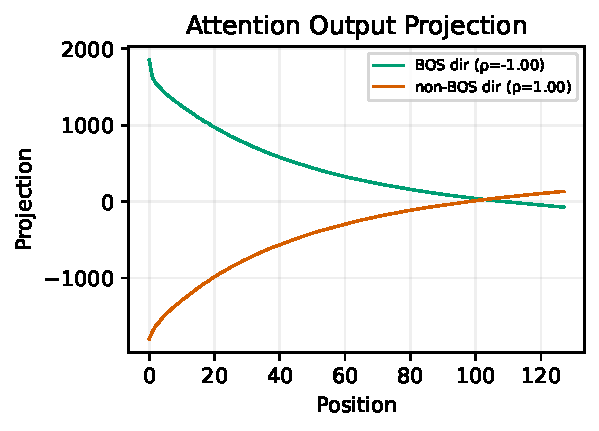
\includegraphics[width=\columnwidth]{plots/r0_attention_output_projection/attention_output_projection_full12h.pdf}
\caption{\textbf{Attention 2 output scalar product with the BOS direction and the non-BOS direction for \modelfull.}}
\label{fig:gauge_projections_full}
\end{figure}

\paragraph{Step 5: Head reads the rotated signal.}
The linear head also aligns with the others direction,
\[
\cos(w_{\text{head}}, d_{\text{nonBOS}})=0.319,
\]

The weaker alignment ($0.32$ vs.\ $0.84$ in \modelminimal) reflects that \modelfull has additional readout pathways: the trained MLP in Block~2 can extract position information beyond the pure attention signal, reducing the head's reliance on direct alignment with $d_{\text{nonBOS}}$.


\paragraph{Summary.}
Across both \modelminimal and \modelfull, we observe a consistent quantitative signature of the five-step geometric gauge:
(i) a structural BOS advantage from causal prefix averaging, (ii) a learned write map that amplifies and separates BOS vs.\ non-BOS directions,
(iii) learned BOS over-attention, (iv) a smooth direction change in the BOS/non-BOS plane that tracks position, and (v) a readout aligned with the non-BOS direction.

\section{Attention maps \modelfull}
\begin{figure}[h]
\centering
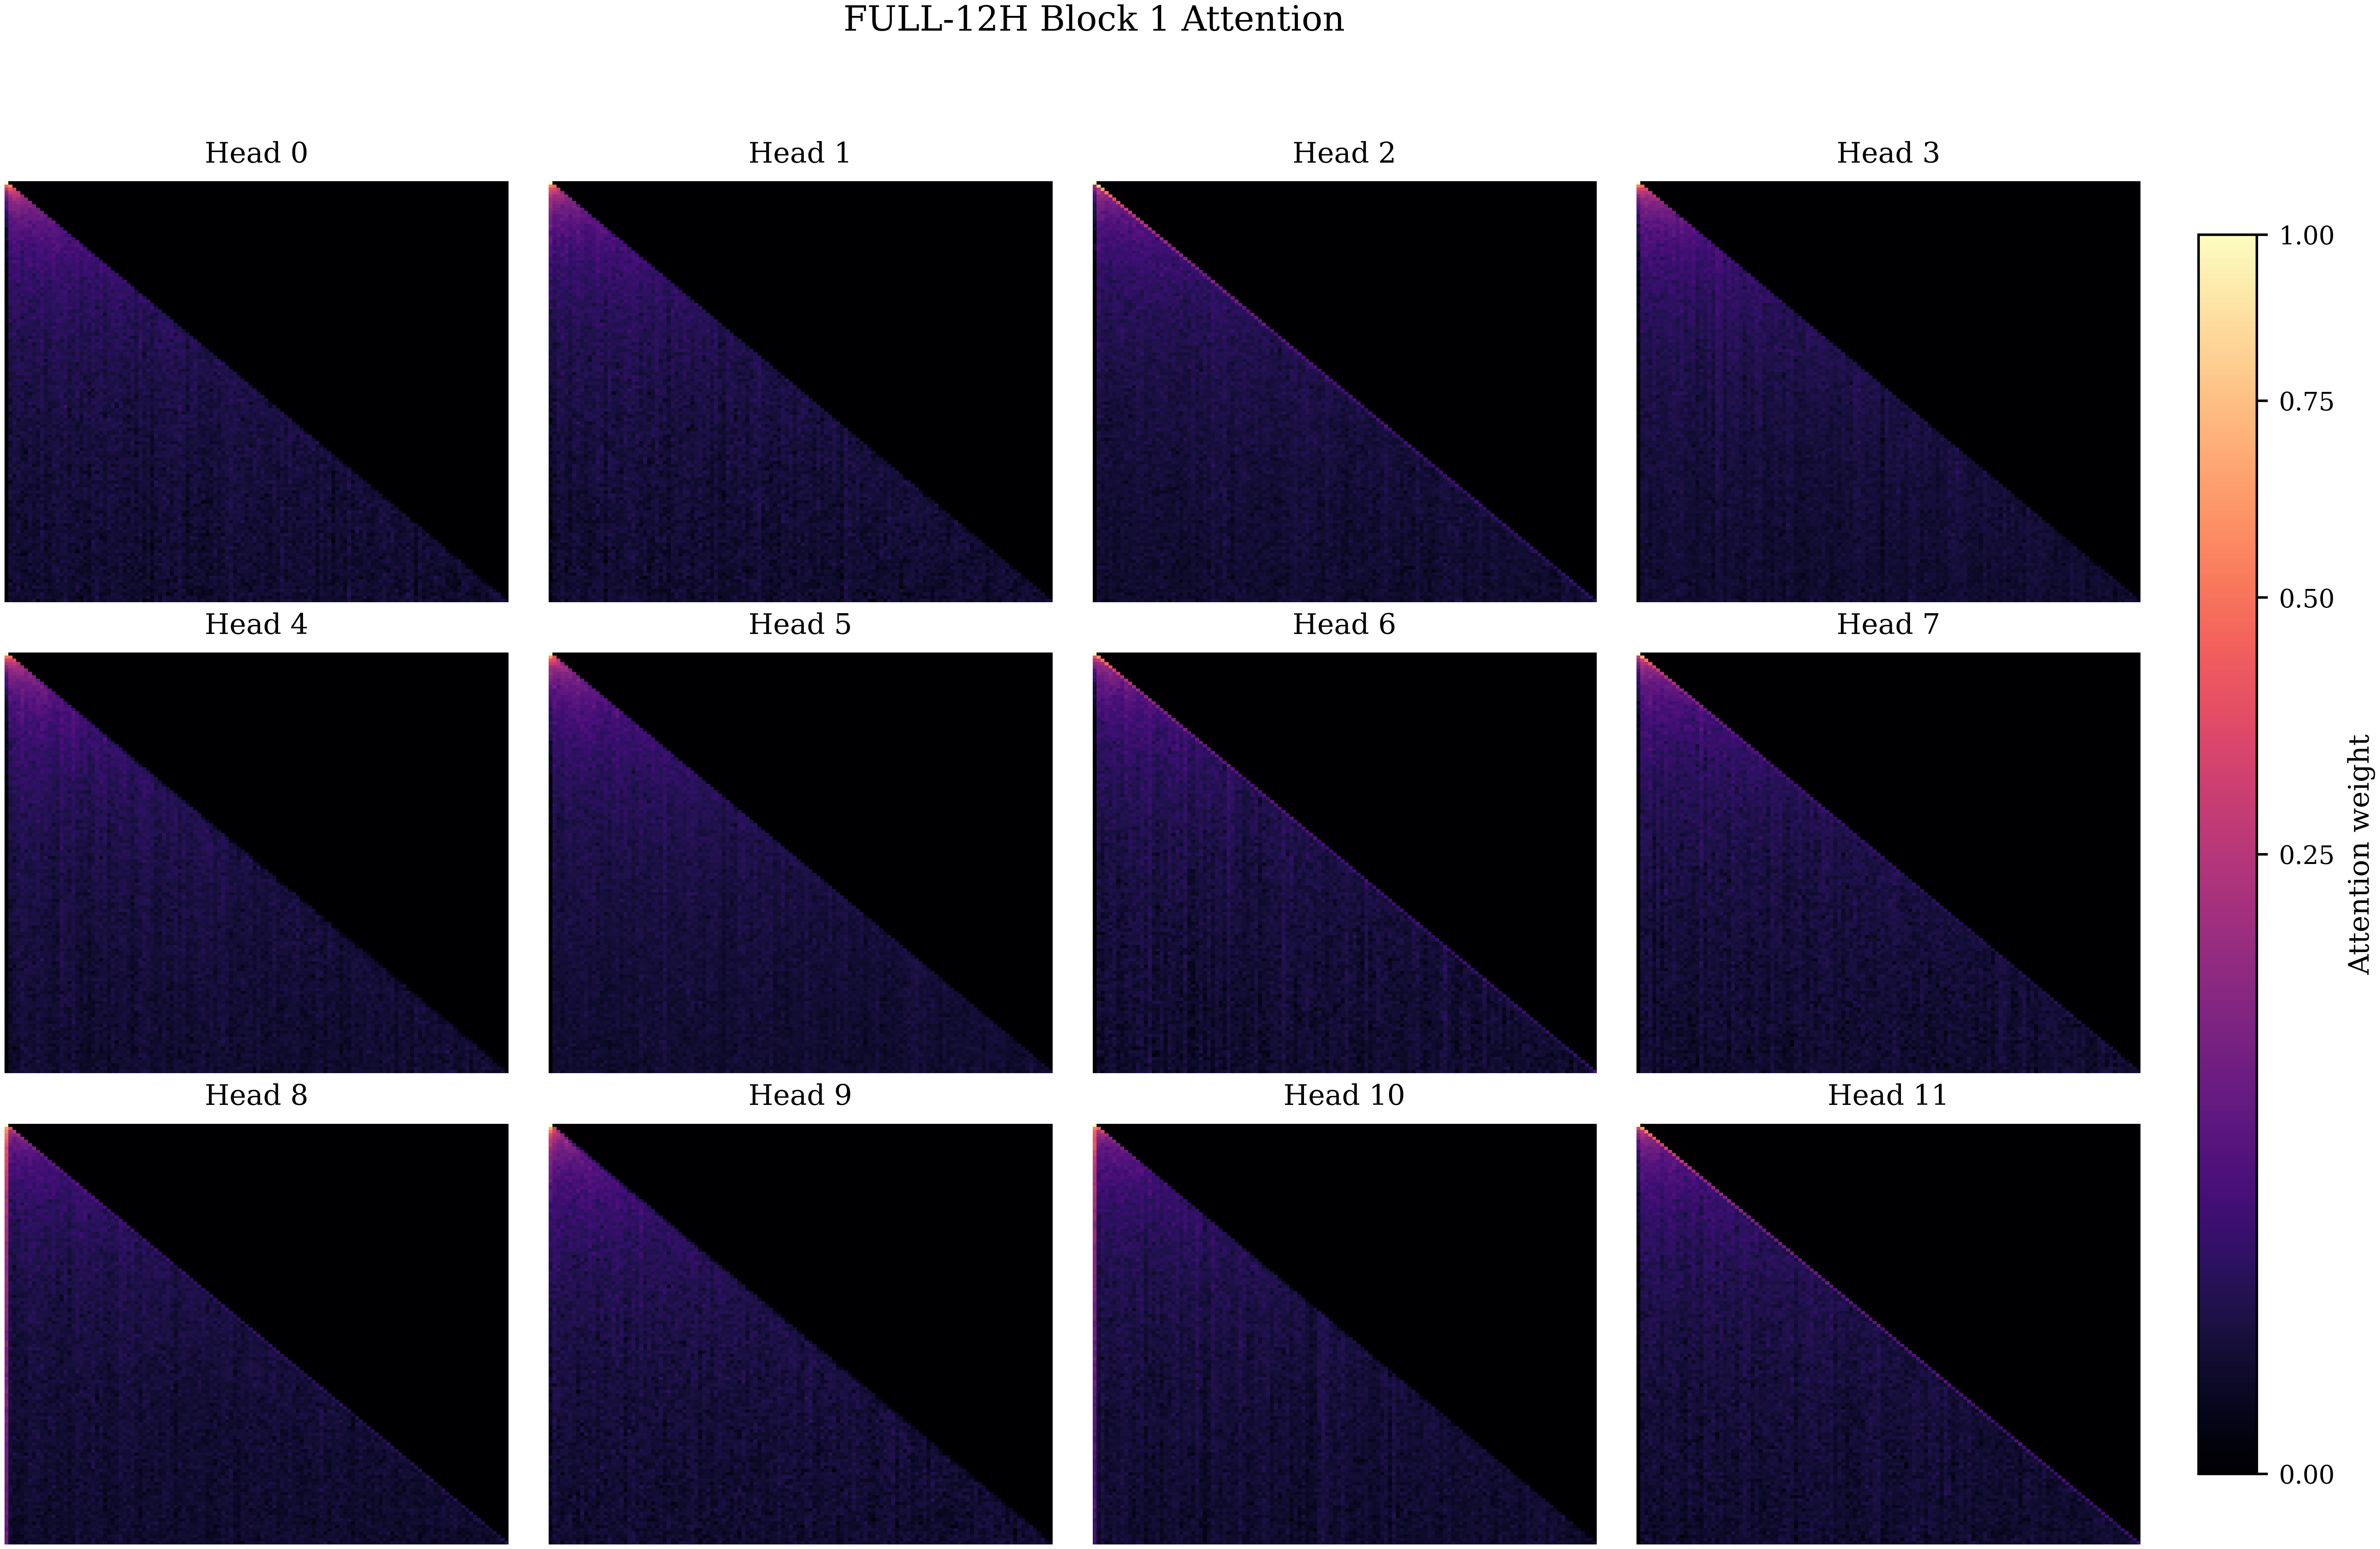
\includegraphics[width=\columnwidth]{plots/attention_uniformity/full12h_block1_attention.png}
\caption{\textbf{\modelfull first block attention masp).}}
\label{fig:full12h_block1_attention}
\end{figure}

\begin{figure}[h]
\centering
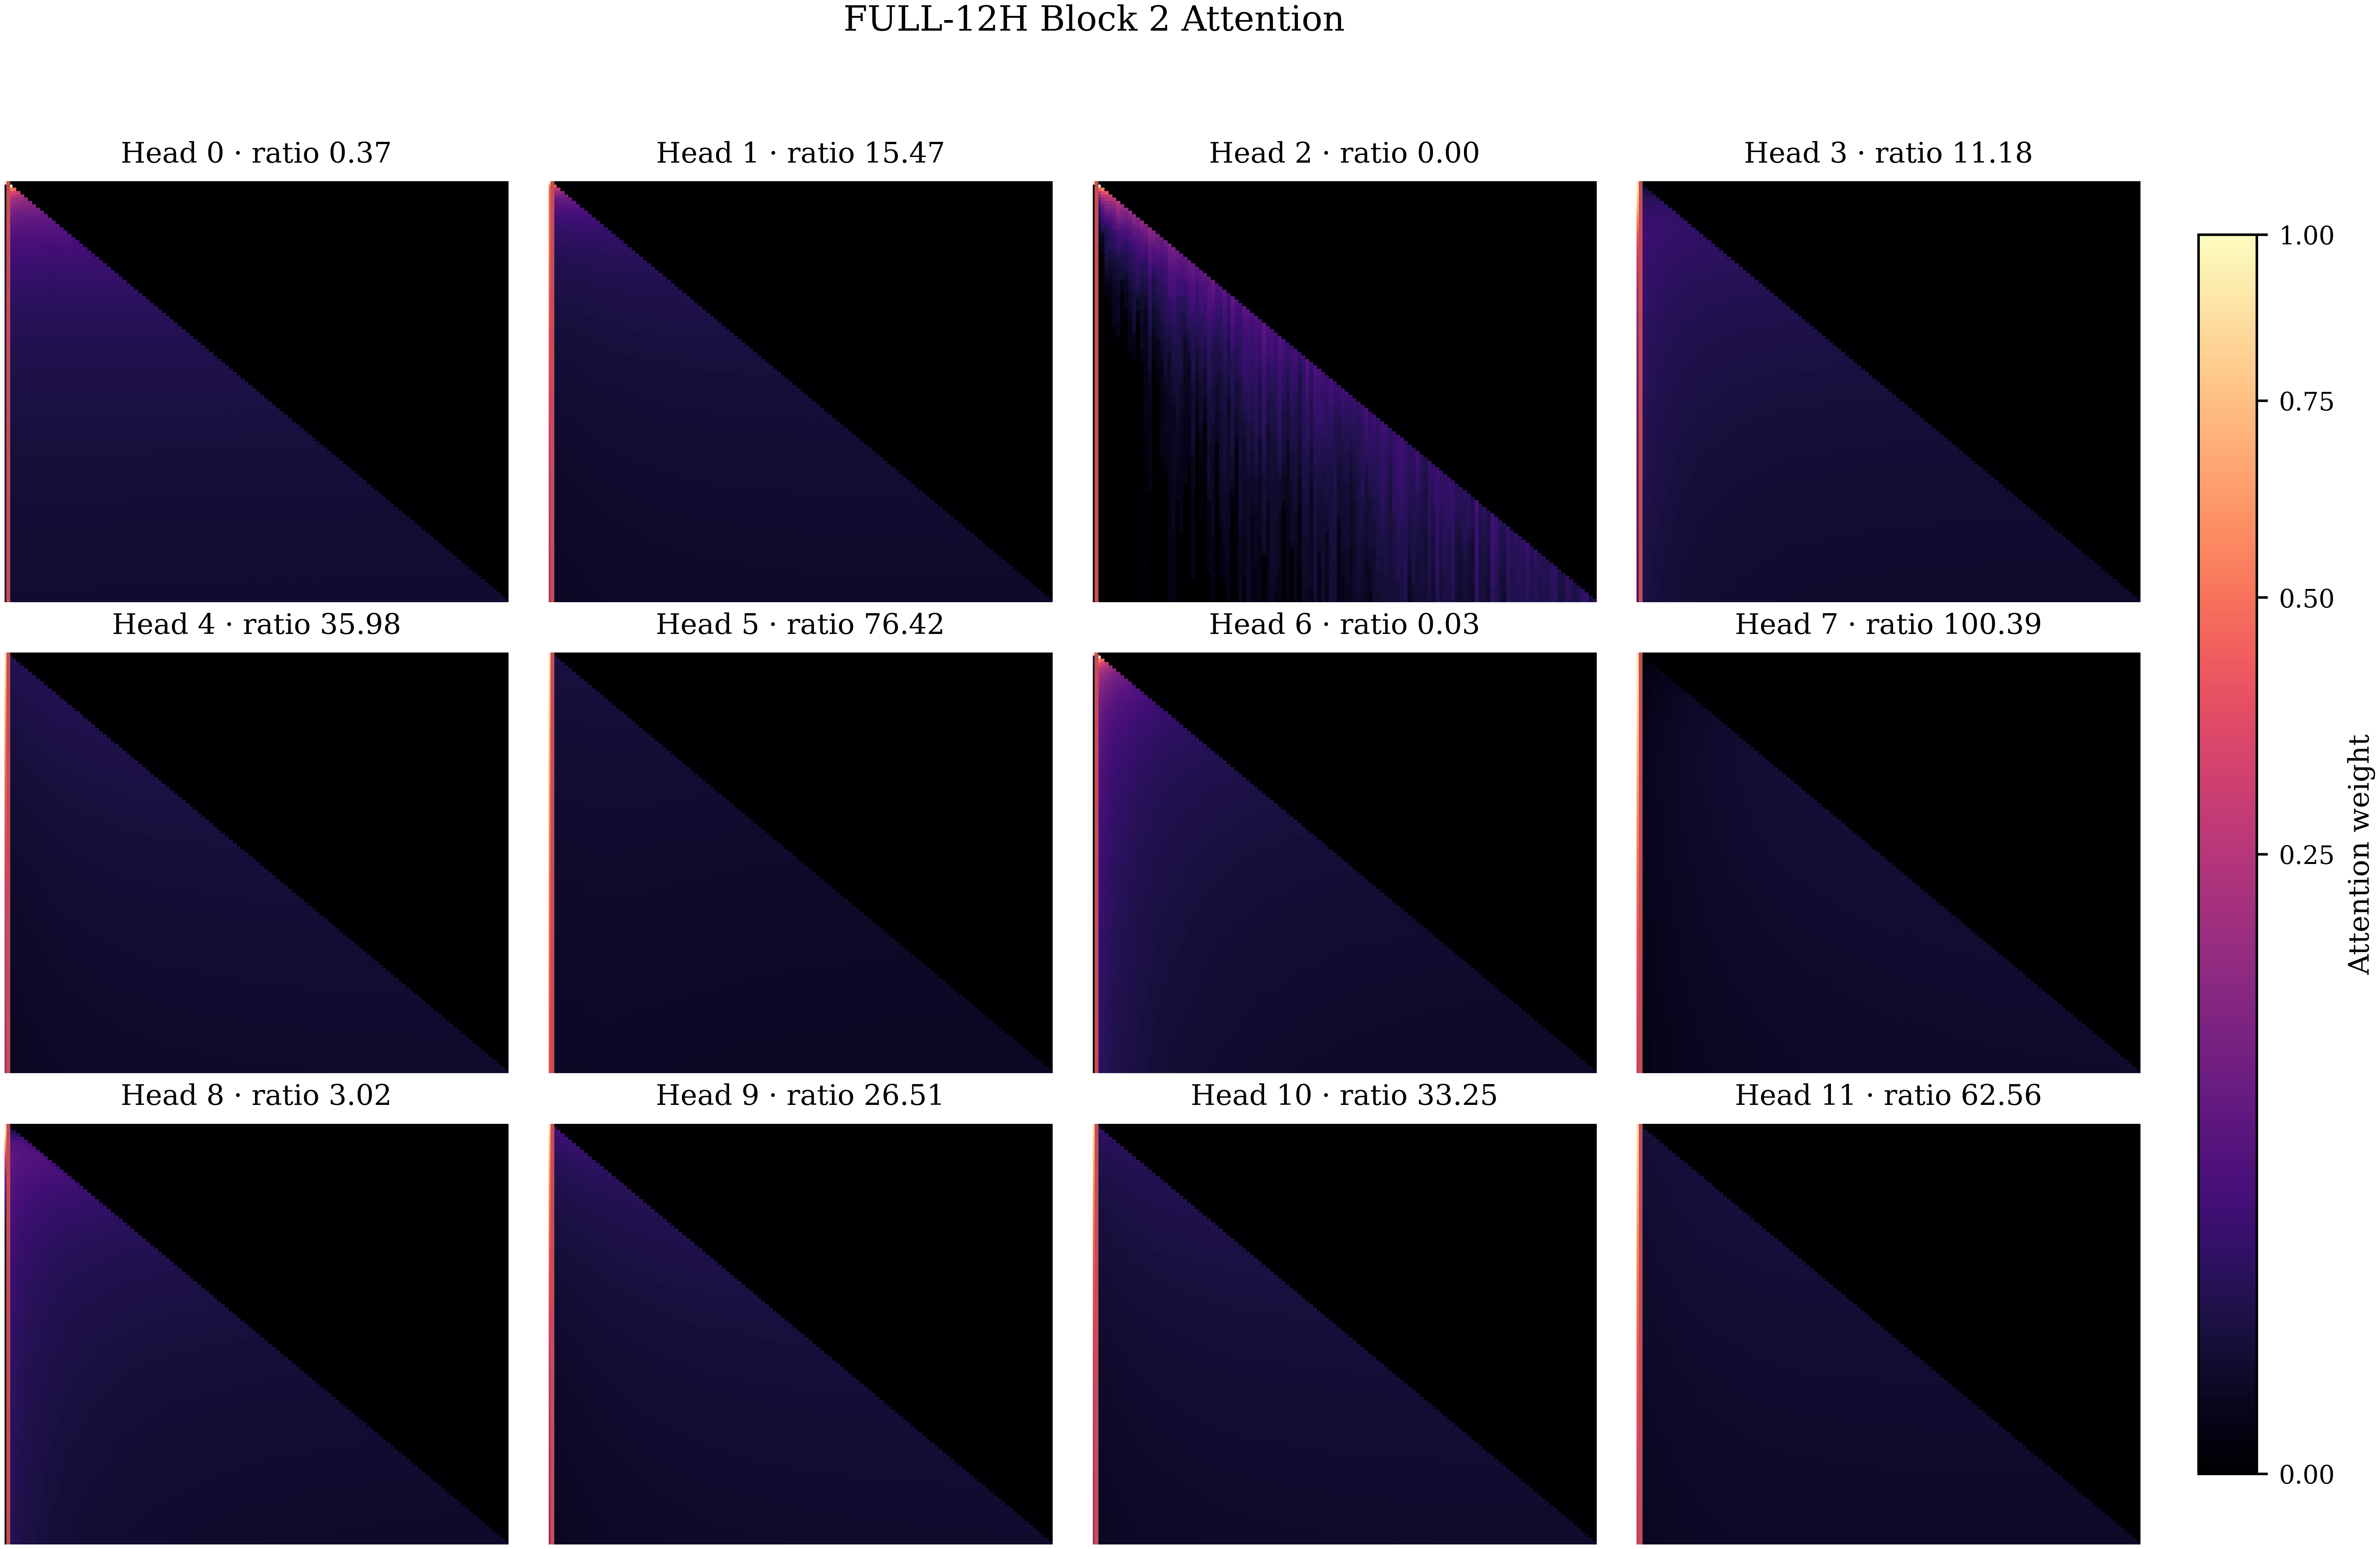
\includegraphics[width=\columnwidth]{plots/attention_uniformity/full12h_block2_attention.png}
\caption{\textbf{\modelfull second block attention masp).}}
\label{fig:full12h_block2_attention}
\end{figure}

\section{Gauge Geometry Demonstration over Individual Sequences}
\begin{figure}[h]
\centering
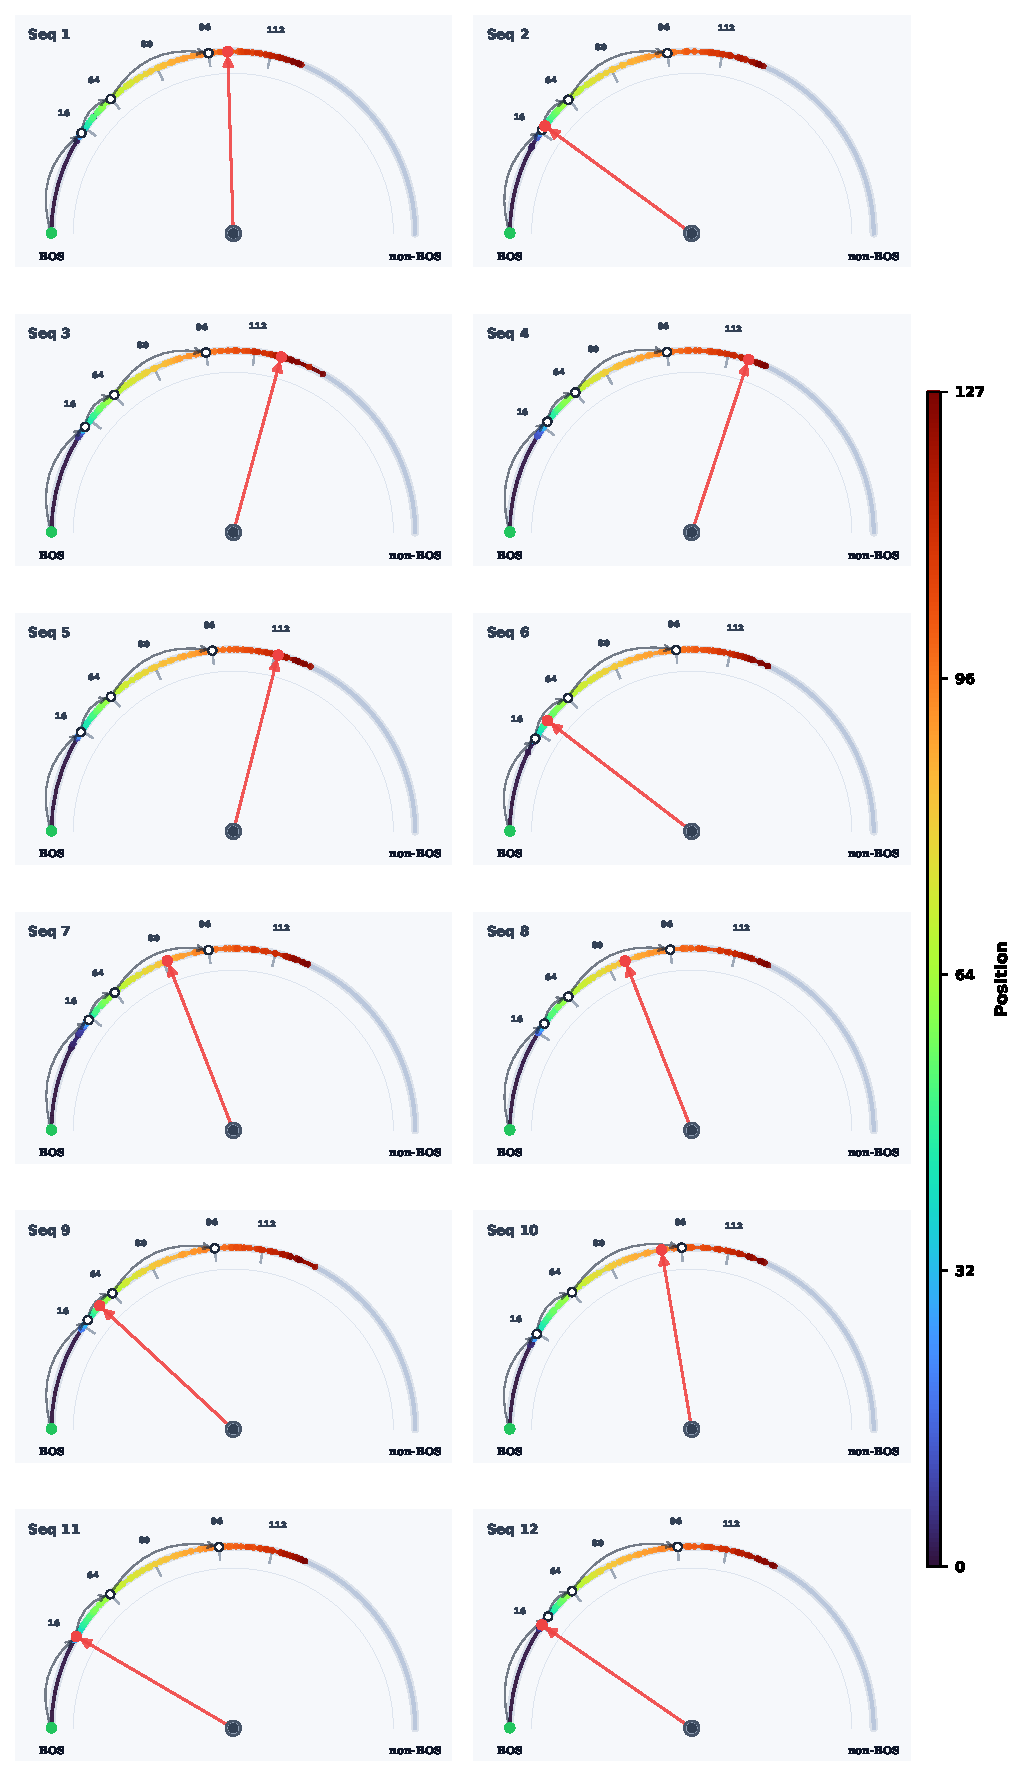
\includegraphics[width=\columnwidth]{plots/r0_directional_rotation_grid.pdf}
\caption{\textbf{Gauge Geometry Demonstration over
Individual Sequences}}
\label{app:gauge_grid}
\end{figure}

\end{document}




